

\section{Introduction}

A large focus of the research on unsteady wings tends towards stall dynamics such as the earlier works of \cite{mccroskey81,mccroskey82experimental,mccroskey73,mccroskey76,carr1977,ericsson_stall88a,ericsson_stall88b}, \emph{etc.} More recent works by \cite{dunne2015,rival2010,choudhry14,visbal11,visbal14,visbal17,alferez13,rosti16} \emph{etc.} continue the investigation which appears far from complete. The review by \cite{mccroskey82} and a more recent one by \cite{coorke15} provide an overview of the dynamic stall process. Much lesser attention has gone towards studying unsteady aerodynamic behavior in the case of small pitch amplitude. Some steadies dealing with small pitch amplitudes include the work done by \cite{pascazio96} which shows a time delay in laminar-turbulent transition during pitching. \cite{nati15} analyzed the effect of small amplitude pitching on a laminar separation bubble at low Reynolds numbers.
\begin{figure}[h]
	\centering
	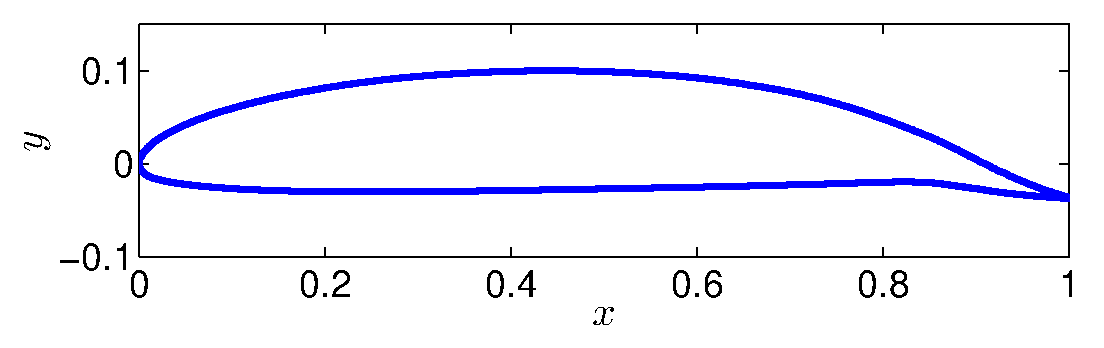
\includegraphics[width=0.95\textwidth]{foil}
	\caption{Natural Laminar Flow (NLF) airfoil tested at the Aeronautical and Vehicle engineering department of KTH \citep{lokatt17,lokattthesis}}
	\label{fig:foil_david}
\end{figure}
Such cases qualitatively represent small changes in operating conditions, such as structural deformations or small trailing edge flap deflections. The understanding of flow response to such changes can be crucial in cases where small perturbations induce large changes in aerodynamic forces. Such sensitive dependence of aerodynamic forces may be found in the static characteristics of natural laminar flow (NLF) airfoils for a certain range of angle of attack. Their performance critically depends on maintaining laminar flow over the suction side of the airfoil and a loss of laminar flow over the airfoil causes large variations of the aerodynamic forces. In addition to such sensitive dependence of the aerodynamic characteristics, recent transonic unsteady experiments using NLF airfoils have brought to light a peculiar property of these airfoils. The unsteady aerodynamic coefficients exhibit a non-linear dynamic response to simple harmonic pitch motions \cite{mai11,hebler13}. Such a non-linear response is inconsistent with the predictions of classical unsteady aerodynamic models \citep{theodorsen35}. Similar experiments within the subsonic range have been performed by \cite{lokattthesis} who also found strongly non-linear behavior of the normal force coefficient. These non-linearities occur only for oscillations within a certain range of angle of attack ($\alpha$) and have been strongly linked to the free movement of transition over the suction side of the airfoil. They seem to be nearly absent when suction side transition is fixed at the leading-edge \citep{mai11,lokattthesis}. 

The present work investigates the effect of small-amplitude pitch oscillations on one such laminar airfoil (figure~\ref{fig:foil_david}). The airfoil was designed at the Aeronautical and Vehicle Engineering department of KTH, where it has been used in a wide range of experimental and numerical work \citep{lokatt17}. The same airfoil was used in the unsteady experiments of \cite{lokattthesis}. The simulations are performed at a chord-based Reynolds number of $Re_{c}=100,000$. The angle of attack range for the oscillation was chosen from the static characteristics of the airfoil. The static characteristics were calculated using an integral boundary layer code, XFOIL \citep{drela89}, which predicted sharp changes in the coefficient of moment ($C_{m}$) and suction side transition location (figure~\ref{fig:xfoil_cm}) above an angle of attack $\alpha>6^{\circ}$. The steep slope of the coefficient of moment curve indicates a region of sensitive dependence of aerodynamic forces on $\alpha$. The pitch oscillations are performed within this sensitive region.
\begin{figure}[h]
	\centering
	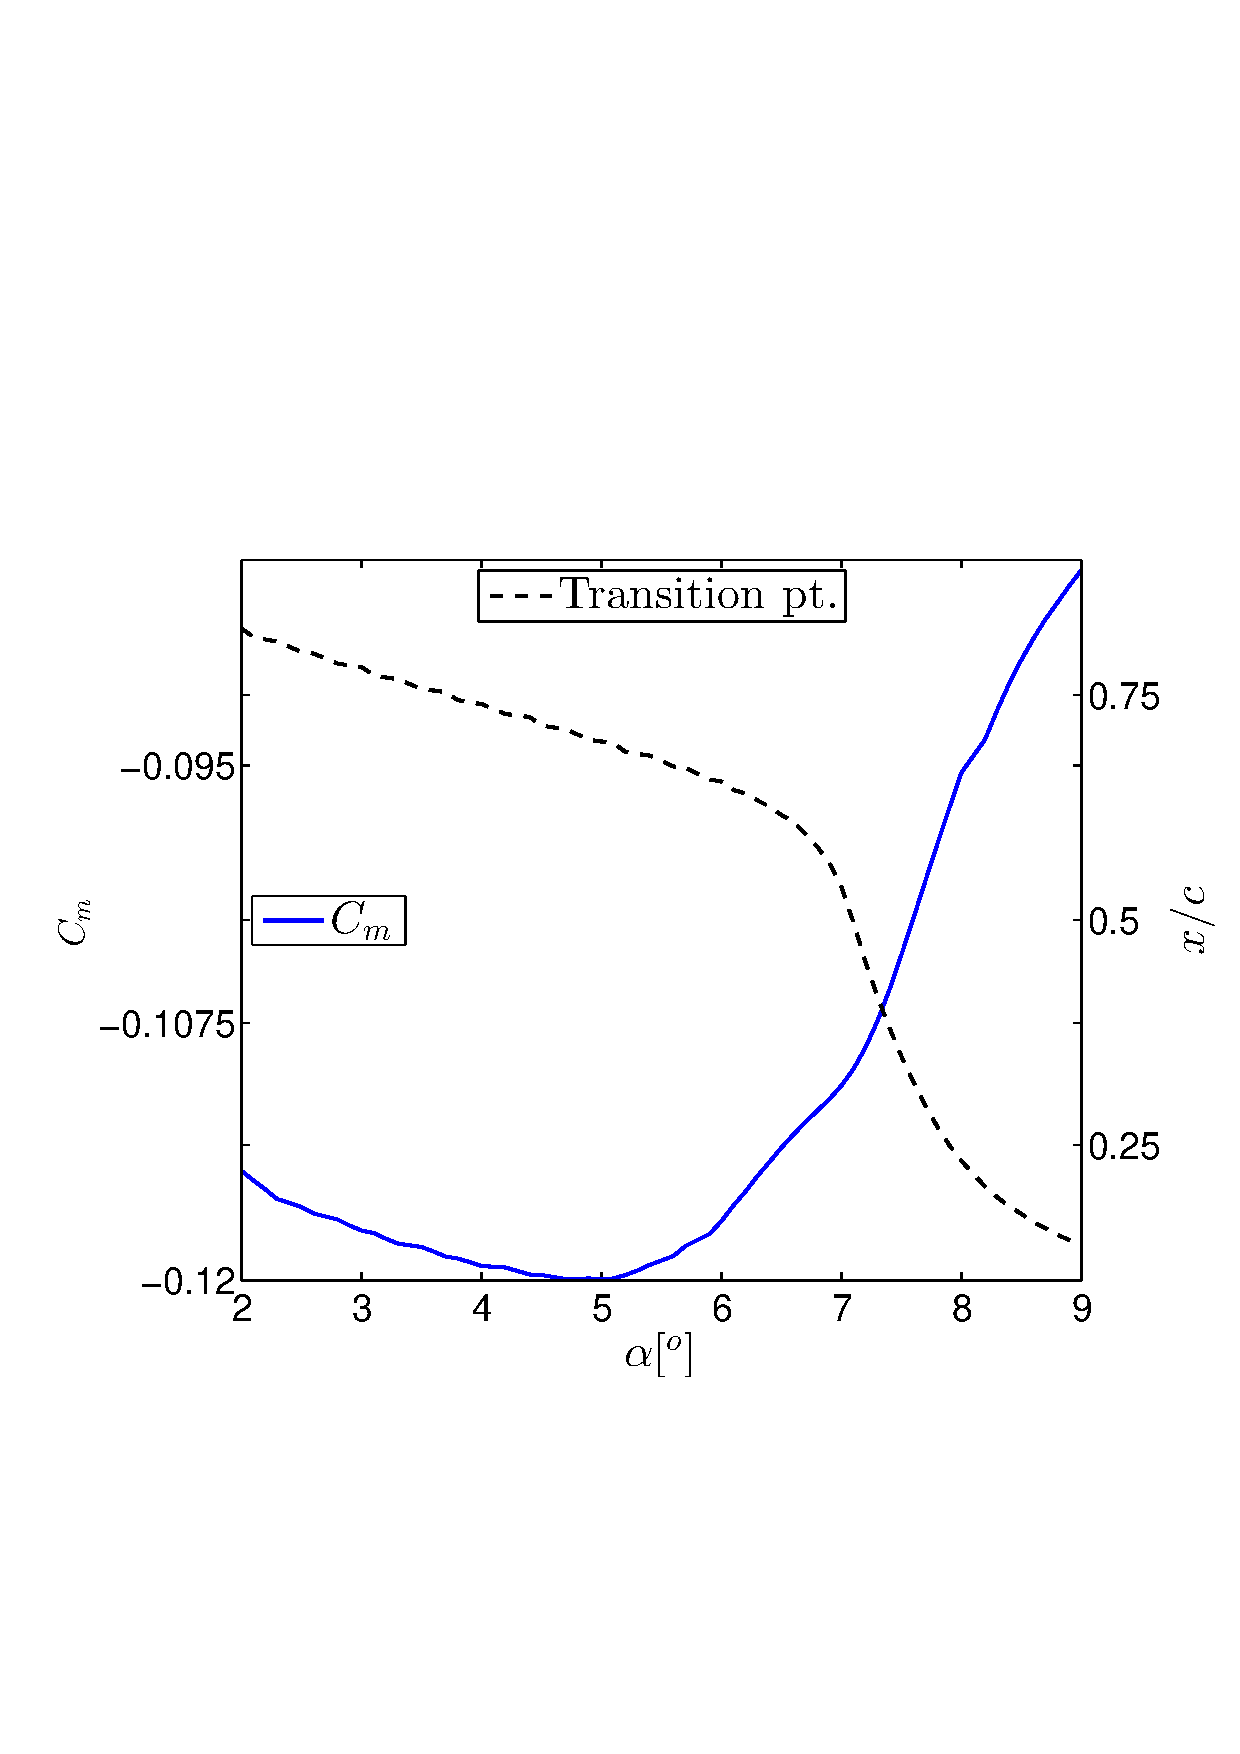
\includegraphics[width=0.75\textwidth]{cm-tr-xfoil_re100k}
	\caption{Coefficient of moment ($C_{m}$) (values on the left axis), and suction side transition location (values on the right axis) as calculated using XFOIL.}
	\label{fig:xfoil_cm}
\end{figure}

In recent works, wall-resolved large-eddy simulations have proven to be an effective tool for studying flow physics at high Reynolds numbers with a computational cost which is much lower than that of direct numerical simulations (DNS). Some of the works to utilize this method include spatially evolving boundary layers \citep{eitel14}, pipe flows \citep{chin15} and flow over wings \citep{uzun10,lombard15}. Successful application of the approach has motivated its use in the present work, which aims to gain insight into the flow-physics of unsteady airfoils undergoing small amplitude pitch oscillations.

The remainder of the paper is divided into 3 sections. Section 2 describes the numerical setup and presents the results of the validation of the LES. Results of both the stationary and pitching simulations are discussed in Section 3. The conclusions of the study are presented in Section 4.

\section{Computational setup}

\subsection{Numerical method}

The computational code used for the simulations is Nek5000, which is an open-source incompressible Navier--Stokes solver developed by \cite{nek5000} at Argonne National Laboratory. It is a based on a spectral-element method which allows the mapping of elements to complex geometries along with a high-order spatial discretization within the elements. The method uses Lagrange interpolants as basis functions and utilizes Gauss--Lobatto--Legendre (GLL) quadrature for the distribution of points within the elements. The spatial discretization is done by means of the Galerkin approximation, following the $P_{N}-P_{N-2}$ formulation. An $11^{th}$ order polynomial approximation is used for the velocity with a $9^{th}$ order approximation for pressure. The nonlinear terms are treated explicitly by third-order extrapolation (EXT3), whereas the viscous terms are treated implicitly by a third-order backward differentiation scheme (BDF3). Aliasing errors are removed with the use of over-integration. All equations are solved in non-dimensional units with the velocities normalized by the reference free-stream velocity $U_{0}$ and the length scales in all directions are normalized by the chord length $c$. The resultant non-dimensional time unit is given by $c/U_{0}$.
%%%%%%%%%%%%%%%%%%%%%%%%%%%%%%%%%%%%%%%%%%%%%%%%%%%%%%%%%%%%%%%%%%%%%%
\subsection{Relaxation-term large-eddy simulation (RT-LES)}

The LES method is based on the RT3D variant of the ADM-RT approach first used by \cite{schlatter04}. The method supplements the governing equations with a dissipative term ($\chi\mathcal{H}(u)$). The equations for the resolved velocity and pressure thus read:
\begin{subequations}
	\begin{eqnarray}
		\frac{\partial u}{\partial t} + u\cdot\nabla u =  - \frac{1}{\rho}\nabla p + \frac{1}{Re}\nabla^{2}u -\chi\mathcal{H}(u), \\
		\nabla\cdot u = 0,
	\end{eqnarray}
\end{subequations}
where $\mathcal{H}$ is a defined high-pass spectral filter and $\chi$ is a model parameter. Together the two parameters determine the strength of the dissipative term. The method has been used in earlier studies of spatially developing boundary layers \citep{eitel14} and channel flows \citep{schlatter06}, and has been shown to be reliable in predicting transition location and also preserving the characteristic structures which are seen in the DNS of transitional flows by \cite{schlatter06}.

A number of tests were carried out in a channel flow at a friction Reynolds number of $Re_{\tau}=395$, and the results are compared with the DNS data of \cite{moser99}. The final mesh was set up such that the streamwise resolution was $\Delta x^{+}=18$ and the spanwise resolution was $\Delta z^{+}=9$. The first point in the wall-normal direction was set at $\Delta y_{w}^{+}=0.64$ and the wall-normal resolution near the boundary layer edge was $y_{max}^{+}=11$. The superscript $^{+}$ indicates normalization in inner units. The resolution is very similar to the one used in \cite{eitel14} where the ADM-RT model is used to simulate a spatially evolving boundary layer. A comparison of the results for the turbulent channel flow is shown for the mean velocity in figure~\ref{fig:vel_mean}, and for the turbulent kinetic energy (TKE) budget in figure~\ref{fig:budget}. The dissipation profile shown in the figure is the sum of resolved dissipation and the added dissipation by the relaxation term. A very good agreement with the DNS is found for the mean velocity and all the kinetic energy budget terms (including the total dissipation).

\begin{figure}[h]
	\begin{subfigure}[t]{0.5\textwidth}
		\centering
		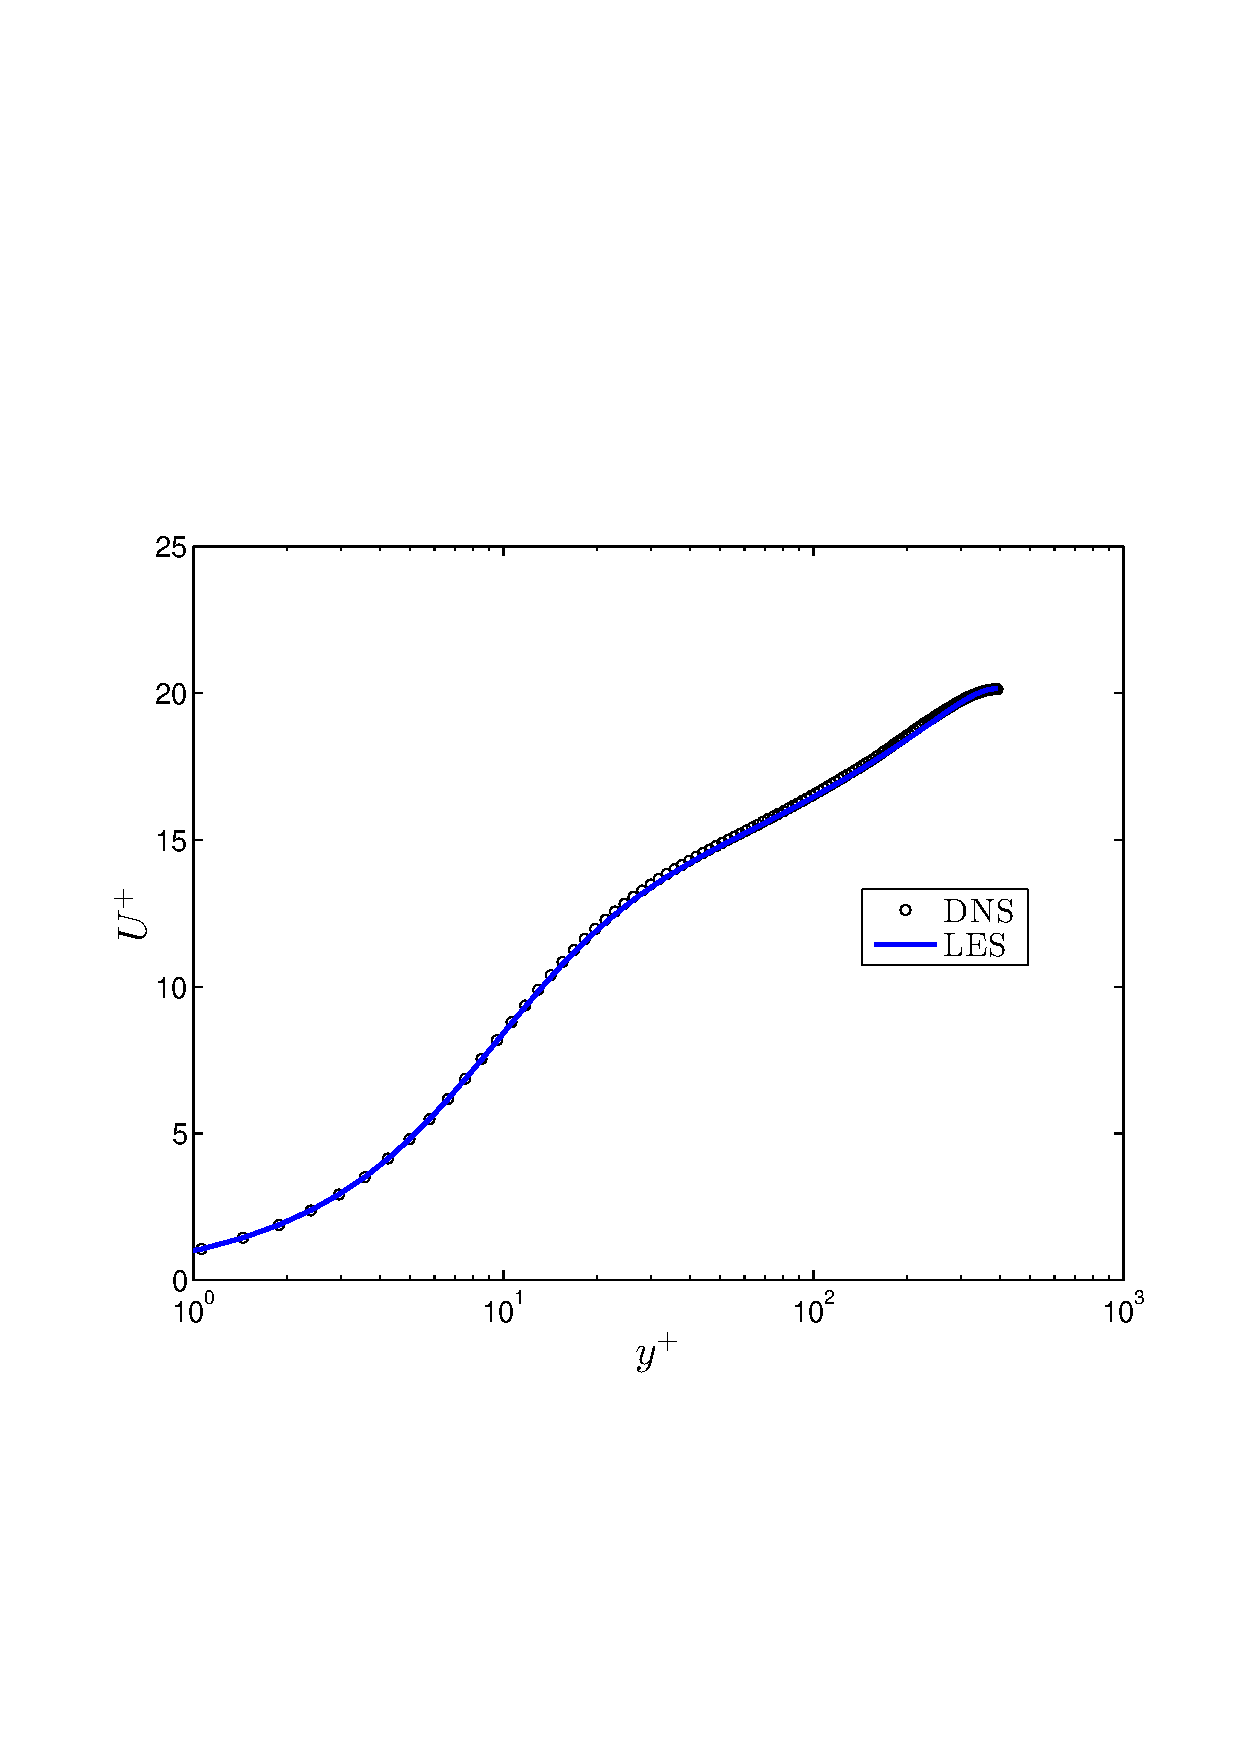
\includegraphics[width=0.95\textwidth]{vel-log}
		\caption{Mean velocity profile.}
		\label{fig:vel_mean}
	\end{subfigure}	
	\begin{subfigure}[t]{0.5\textwidth}
		\centering
		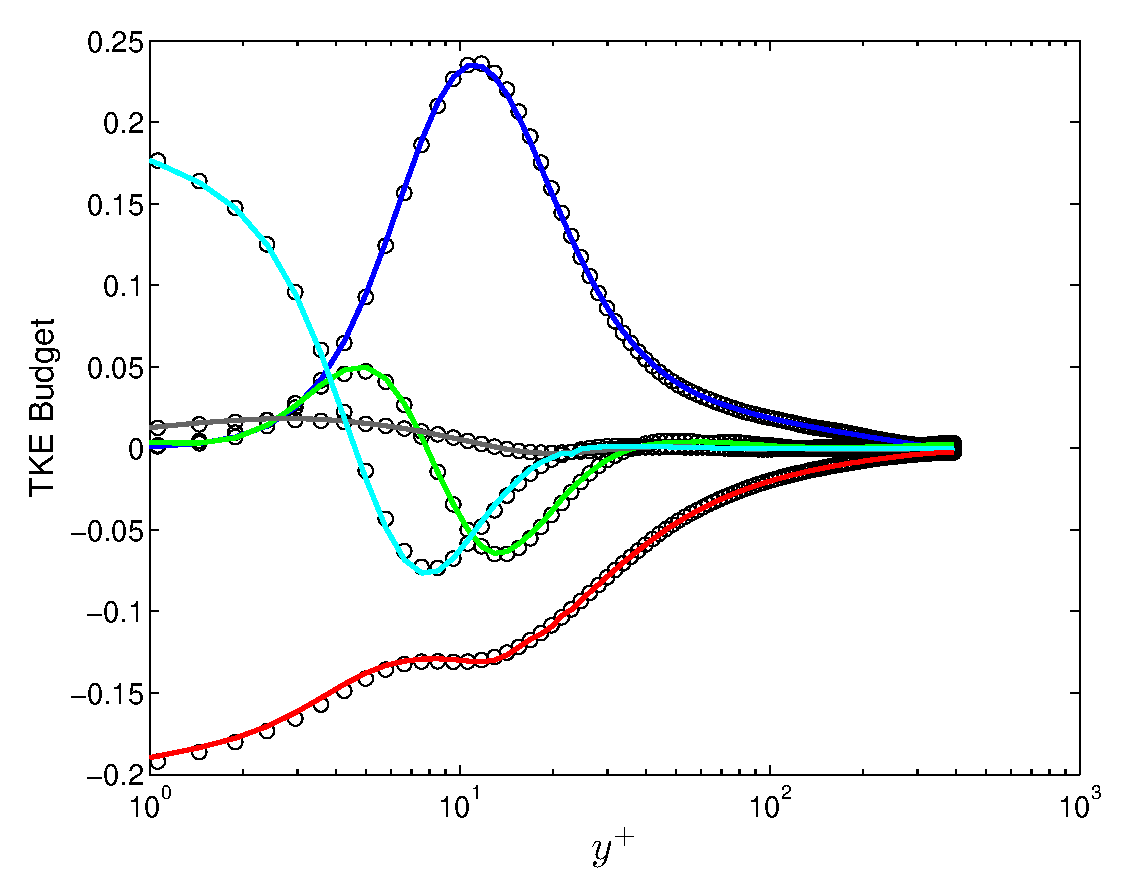
\includegraphics[width=0.98\textwidth]{budgets}
		\caption{Turbulent kinetic energy budget}
		\label{fig:budget}
	\end{subfigure}
	\caption{Comparison of mean velocity profile and turbulent kinetic energy budget. Circles represent the DNS data from \cite{moser99} while the lines represent the values from the LES. All values are normalized with inner units. The individual terms are color coded as: Production (\textcolor{blue}{blue}), dissipation (\textcolor{red}{red}), viscous diffusion (\textcolor{cyan}{cyan}), turbulent diffusion (\textcolor{green}{green}), velocity-pressure correlation (\textcolor{mygray}{gray})}
\end{figure}

\begin{figure}[h]
	\centering
	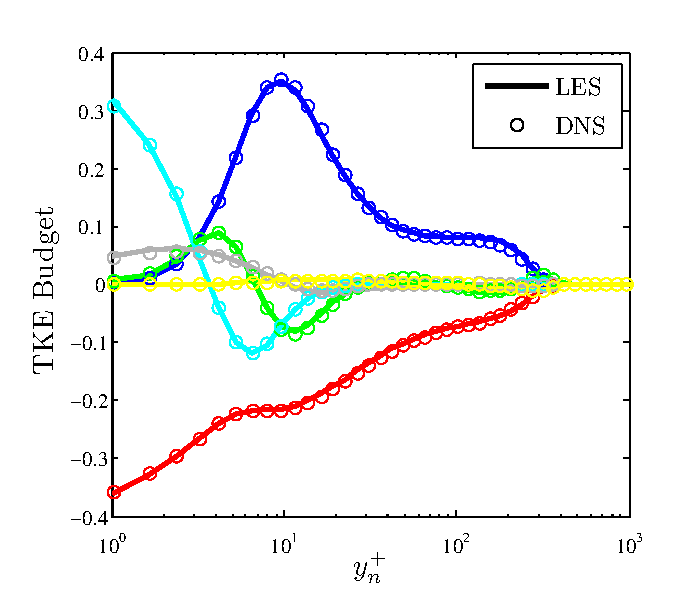
\includegraphics[width=0.6\textwidth]{tke_vs_yp.pdf}
	\caption{Comparison of turbulent kinetic energy budget for a NACA4412 wing section at the suction side location of $x/c=0.7$. The circles represent DNS data from \cite{hosseini16} while the lines are data from the LES. The individual terms are color coded as: Production (\textcolor{blue}{blue}), dissipation (\textcolor{red}{red}), viscous diffusion (\textcolor{cyan}{cyan}), turbulent diffusion (\textcolor{green}{green}), velocity-pressure correlation (\textcolor{mygray}{gray}), convection (\textcolor{yellow}{yellow})}
	\label{fig:wing_budget}
\end{figure}

\subsection{Mesh generation}

The optimum mesh resolution (in inner units) obtained in the channel flow results is then used to design the mesh around the airfoil. Wall-shear stress data is obtained using XFOIL to estimate the grid spacing on the airfoil. A trip is introduced in XFOIL at $x/c\approx0.1$ to obtain turbulent wall-shear values on both the suction and pressure sides of the airfoil. Here $c$ denotes the chord length. Finally, the grid design uses the following criteria:

\begin{itemize}
	\item[$\bullet$] For $0.1<x/c<0.6$, $\Delta x^{+}=18$, $\Delta y_{wall}^{+}=0.64$ and $\Delta y_{max}^{+}=11$, using the local wall-shear ($\tau_{w}$) values on the airfoil. Since the flow is expected to be laminar on the pressure side, the stream-wise resolution is slightly relaxed to $\Delta x^{+}=25$ while keeping the same wall-normal resolution.
	\item[$\bullet$] For $x/c<0.1$, the peak $\tau_{w}$ value over the suction side of the airfoil is used to estimate the grid spacing.
	\item [$\bullet$] For $x/c>0.6$, the suction side experiences a large adverse pressure gradient which significantly reduces $\tau_{w}$ values. Therefore, the $\tau_{w}$ values from the pressure side are used for both the suction and pressure sides.
	\item [$\bullet$] A structured mesh is used, which is extruded in the spanwise direction. Hence the spanwise resolution is constant throughout the domain. The resolution is set to $\Delta z^{+}=9$, where the the peak $\tau_{w}$ value from the suction side is used.
\end{itemize}

\begin{figure}[h]
	\begin{subfigure}[t]{0.49\textwidth}
		\centering
		\caption{}		
		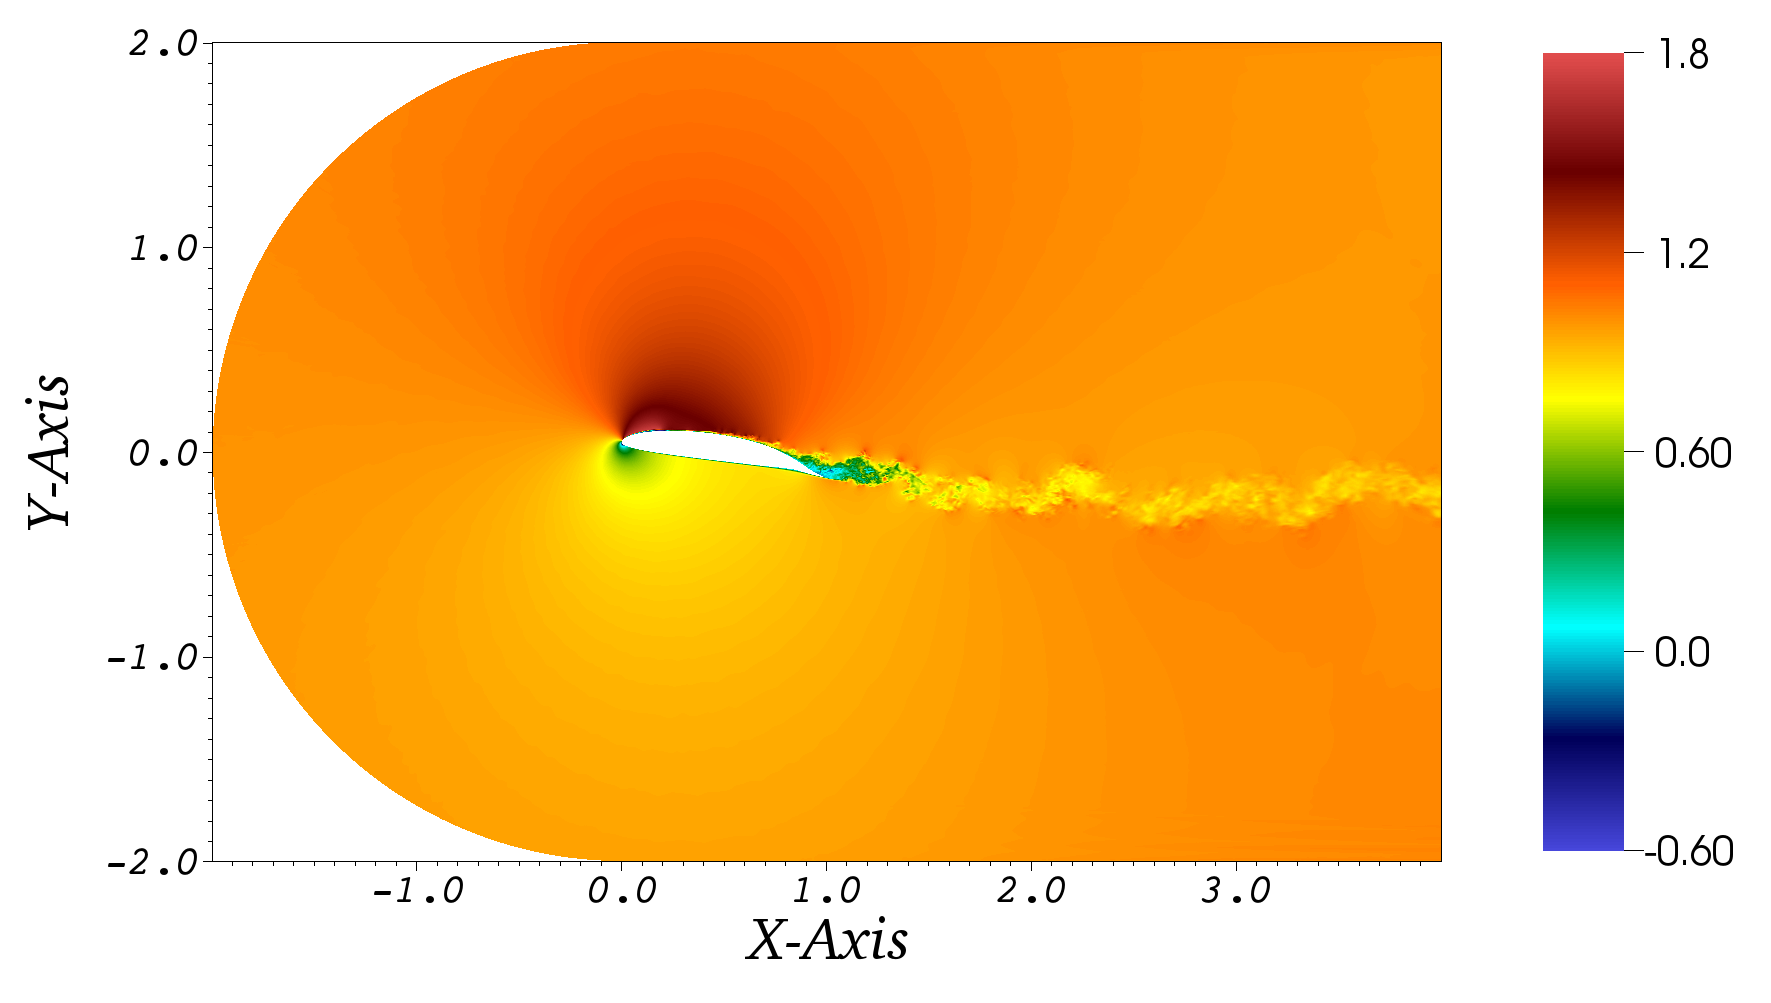
\includegraphics[width=1.0\textwidth]{pitch_re100k0004}
		\label{fig:re100k_domain}
	\end{subfigure}	
	\begin{subfigure}[t]{0.49\textwidth}
		\centering
		\caption{}		
		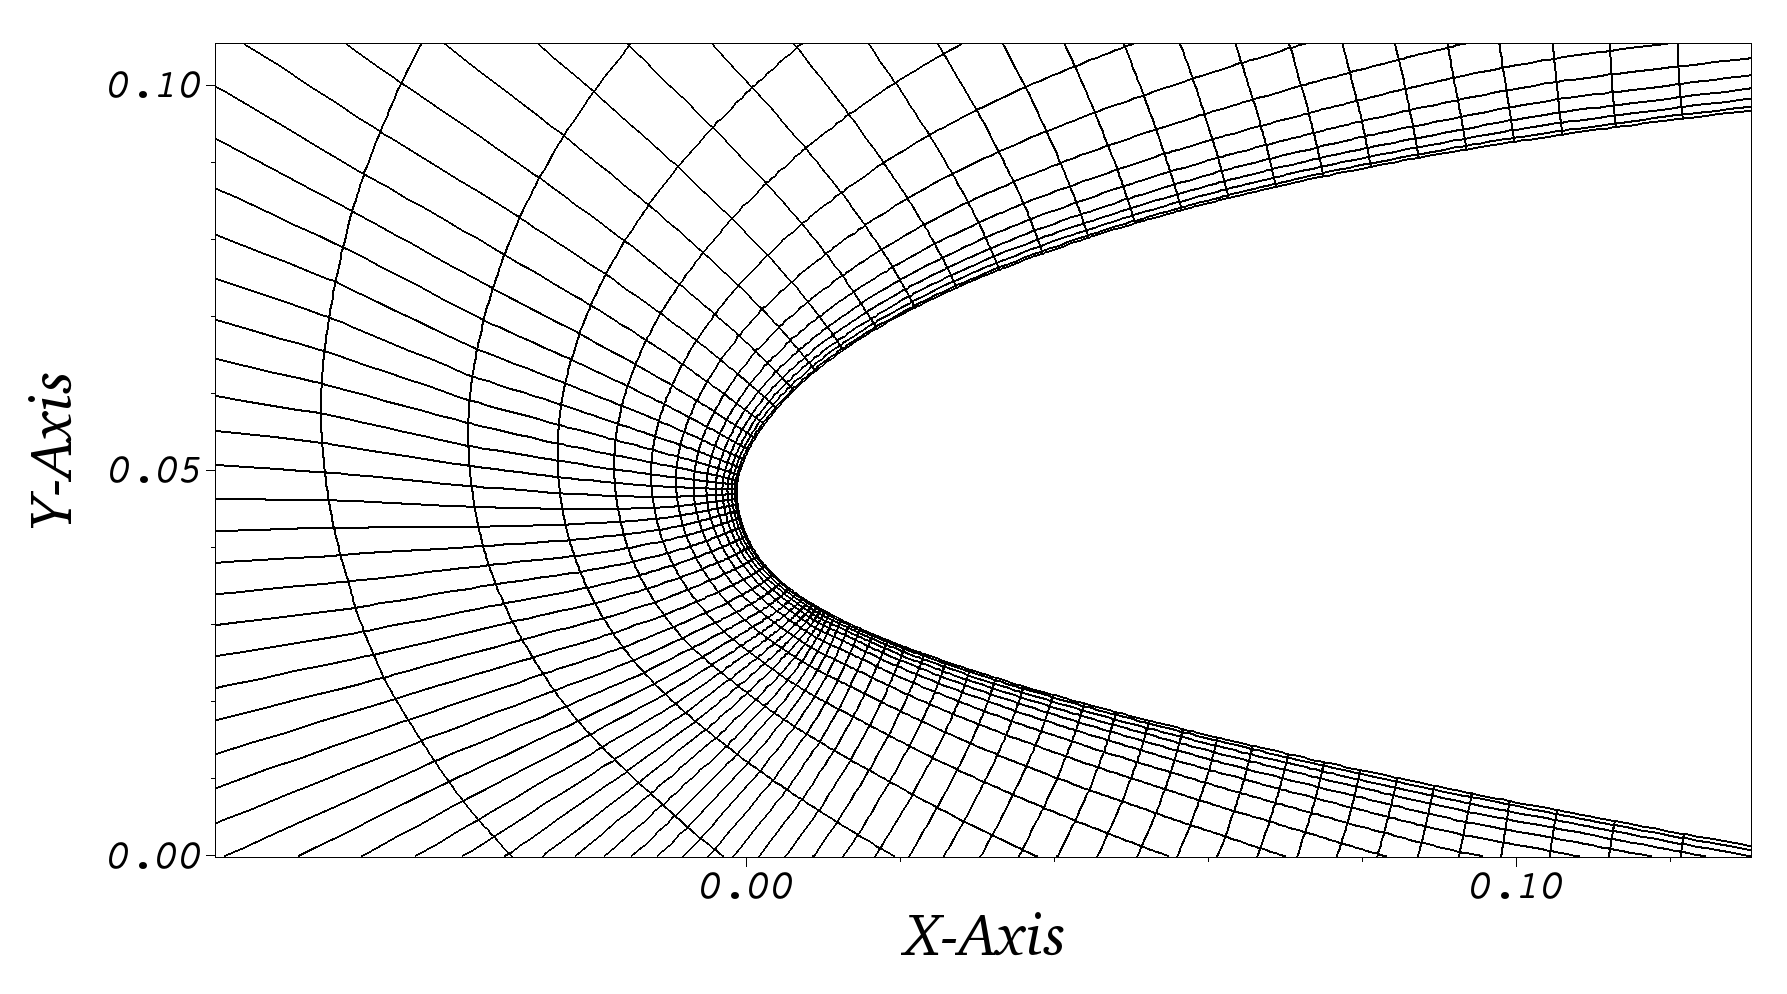
\includegraphics[width=1.\textwidth]{pitch_re100k0003}
		\label{fig:re100k_grid}
	\end{subfigure}
	\caption{(a) 2D section of the simulation domain. Colors represent the instantaneous streamwise velocity. (b) Close-up view of the spectral-element grid near the airfoil surface.}	
\end{figure}

A different criterion is needed for defining the resolution in the wake where the wall-based criteria are not valid. Accordingly, Reynolds-averaged Navier--Stokes (RANS) simulations were performed using the transition $k$-$\Omega$ SST model with \textit{ANSYS}\textsuperscript{\textregistered} FLUENT, to estimate the Kolmogorov length scale ($\eta$) in the wake region. The RANS is setup with domain boundaries at a distance of 100 chords from the airfoil. The grid in the wake region is designed such that the average grid spacing between the GLL points follows the criteria: $\Delta x/\eta < 9$. The computational domain is set up such that the far field boundaries of the computational domain are two chords away from the airfoil leading edge in either direction. The outflow boundary is four chords downstream from the airfoil leading edge and the inlet is designed as a curved inflow boundary with a constant radial distance of two chords from the leading edge of the airfoil. The spanwise width of the domain is $l_{z}=0.25$ chords. The domain can be visualized in figure~\ref{fig:re100k_domain} and a close-up view of the spectral-elements is shown in (figure~\ref{fig:re100k_grid}). Each of the spectral-elements are further discretized by $12\times12\times12$ grid points in 3D, corresponding to an $11^{th}$ order spectral discretization. Periodic boundary conditions are imposed on the spanwise boundaries, while the energy-stabilized outflow condition suggested by \cite{dong2014} is imposed on the outflow boundary. Velocity field data for locations corresponding to the boundaries of the LES computational domain is extracted from an unsteady RANS simulation. The interpolated data is imposed as a Dirichlet boundary condition on these boundaries. The method is very similar to the one used by \cite{hosseini16} in their DNS of flow around a wing section. In order to simulate low turbulence flight conditions, free-stream turbulence of intensity $Ti=0.1\%$ is superimposed on the Dirichlet boundary conditions. The free-stream turbulence is generated using Fourier modes with a von K\'arm\'an spectrum. The procedure is similar to the one described in \cite{schlatterdiploma,brandt04} and \cite{schlatter08} and has been used for the study of transition in flat plate boundary layers under the influence of free-stream turbulence.  

A validation of the above methodology for complex geometries such as a wing section was performed at a chord based Reynolds number of $Re_{c}=400,000$ for NACA4412 airfoil. The LES grid resolution was setup with the same grid criteria as described above. The domain boundaries and boundary conditions are identical to the setup in \cite{hosseini16}. A comparison of the wall-normal profiles of the normalized kinetic energy budget is shown in figure~\ref{fig:wing_budget}. The profiles are extracted a streamwise location of $x/c=0.7$ on the suction side of the airfoil. The LES profiles (lines) match well with the DNS data (circles) of \cite{hosseini16}, signifying the high accuracy of the LES with the current resolution.

\section{Results and discussion}
\subsection{Steady results}
% Aoa 6.7 vs aoa 8.0
\begin{figure}[t]
	\begin{subfigure}[b]{0.49\textwidth}
		\centering
		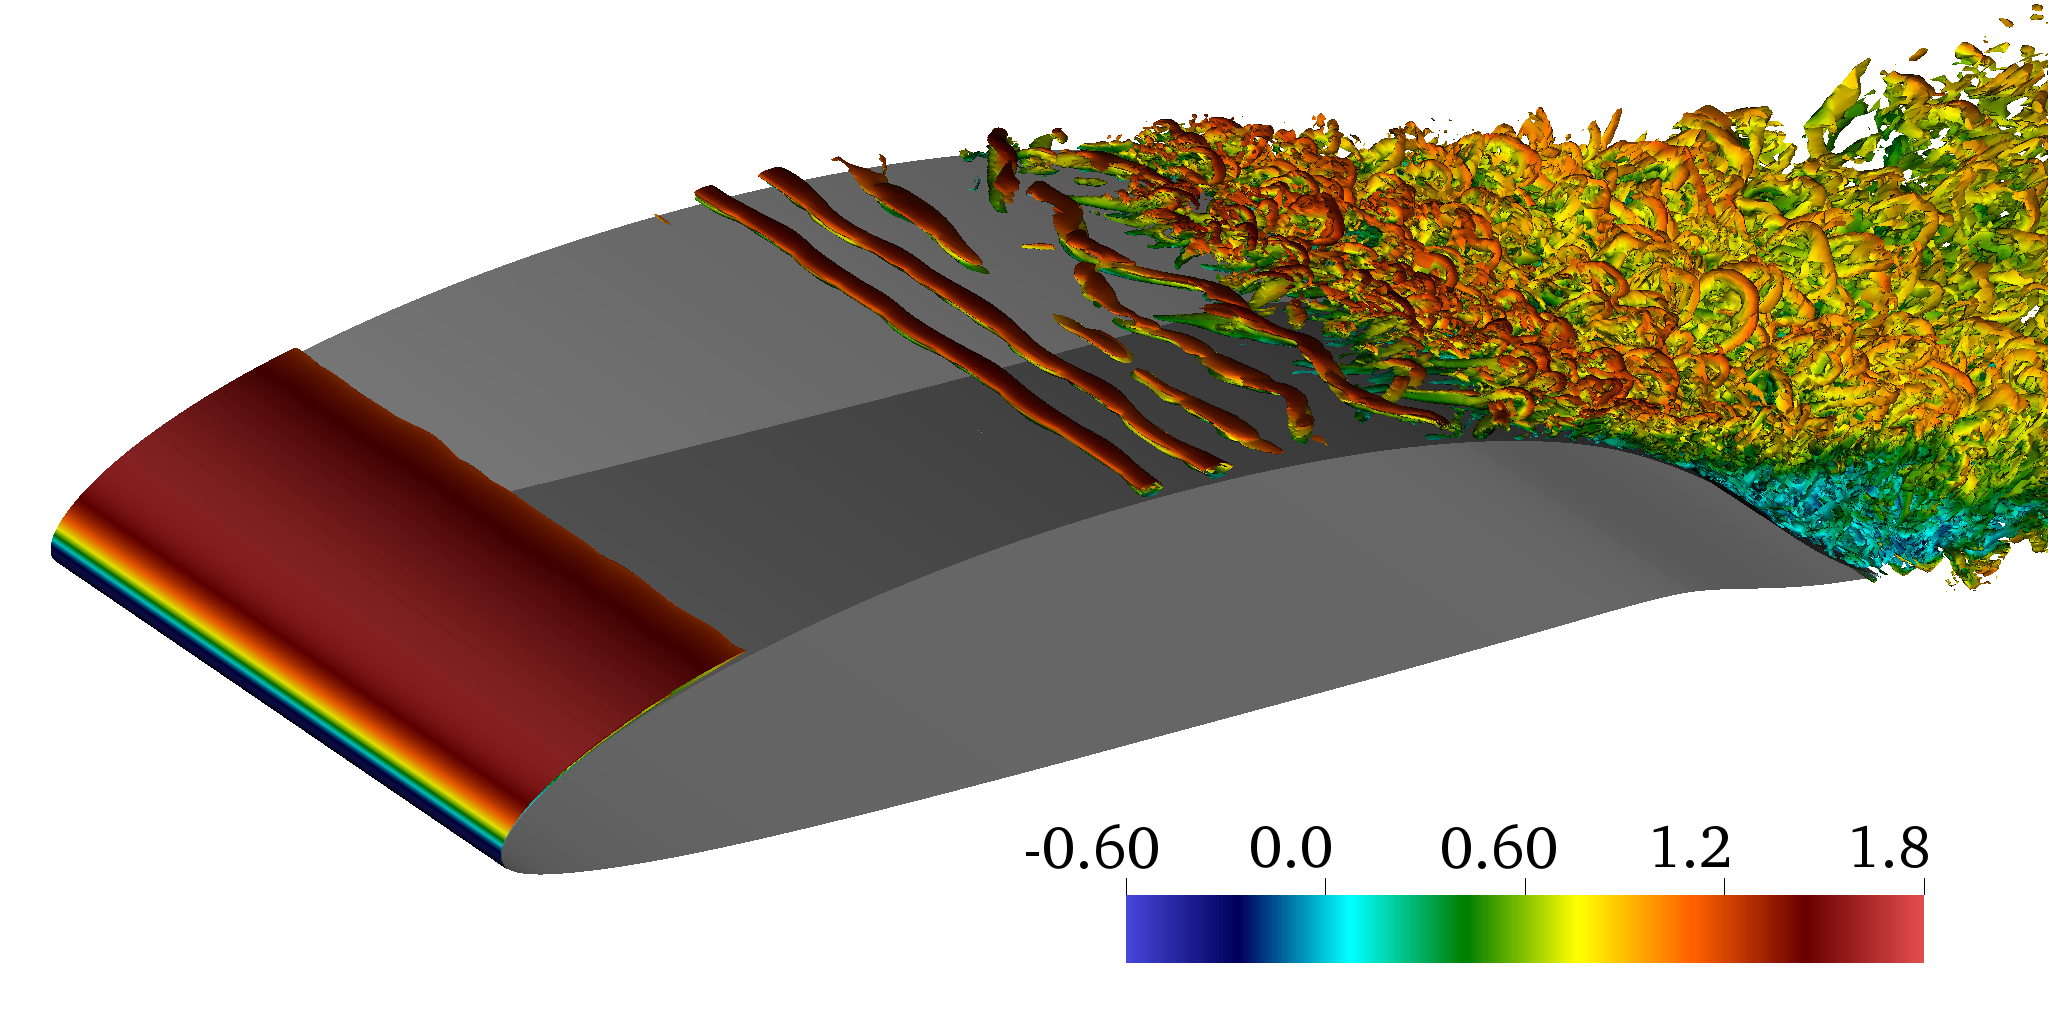
\includegraphics[width=1\textwidth]{re100k_static67_0001}
		\caption{$\alpha=6.7^{\circ}$}
		\label{fig:aoa67_iso}
	\end{subfigure}
	\begin{subfigure}[b]{0.49\textwidth}
		\centering
		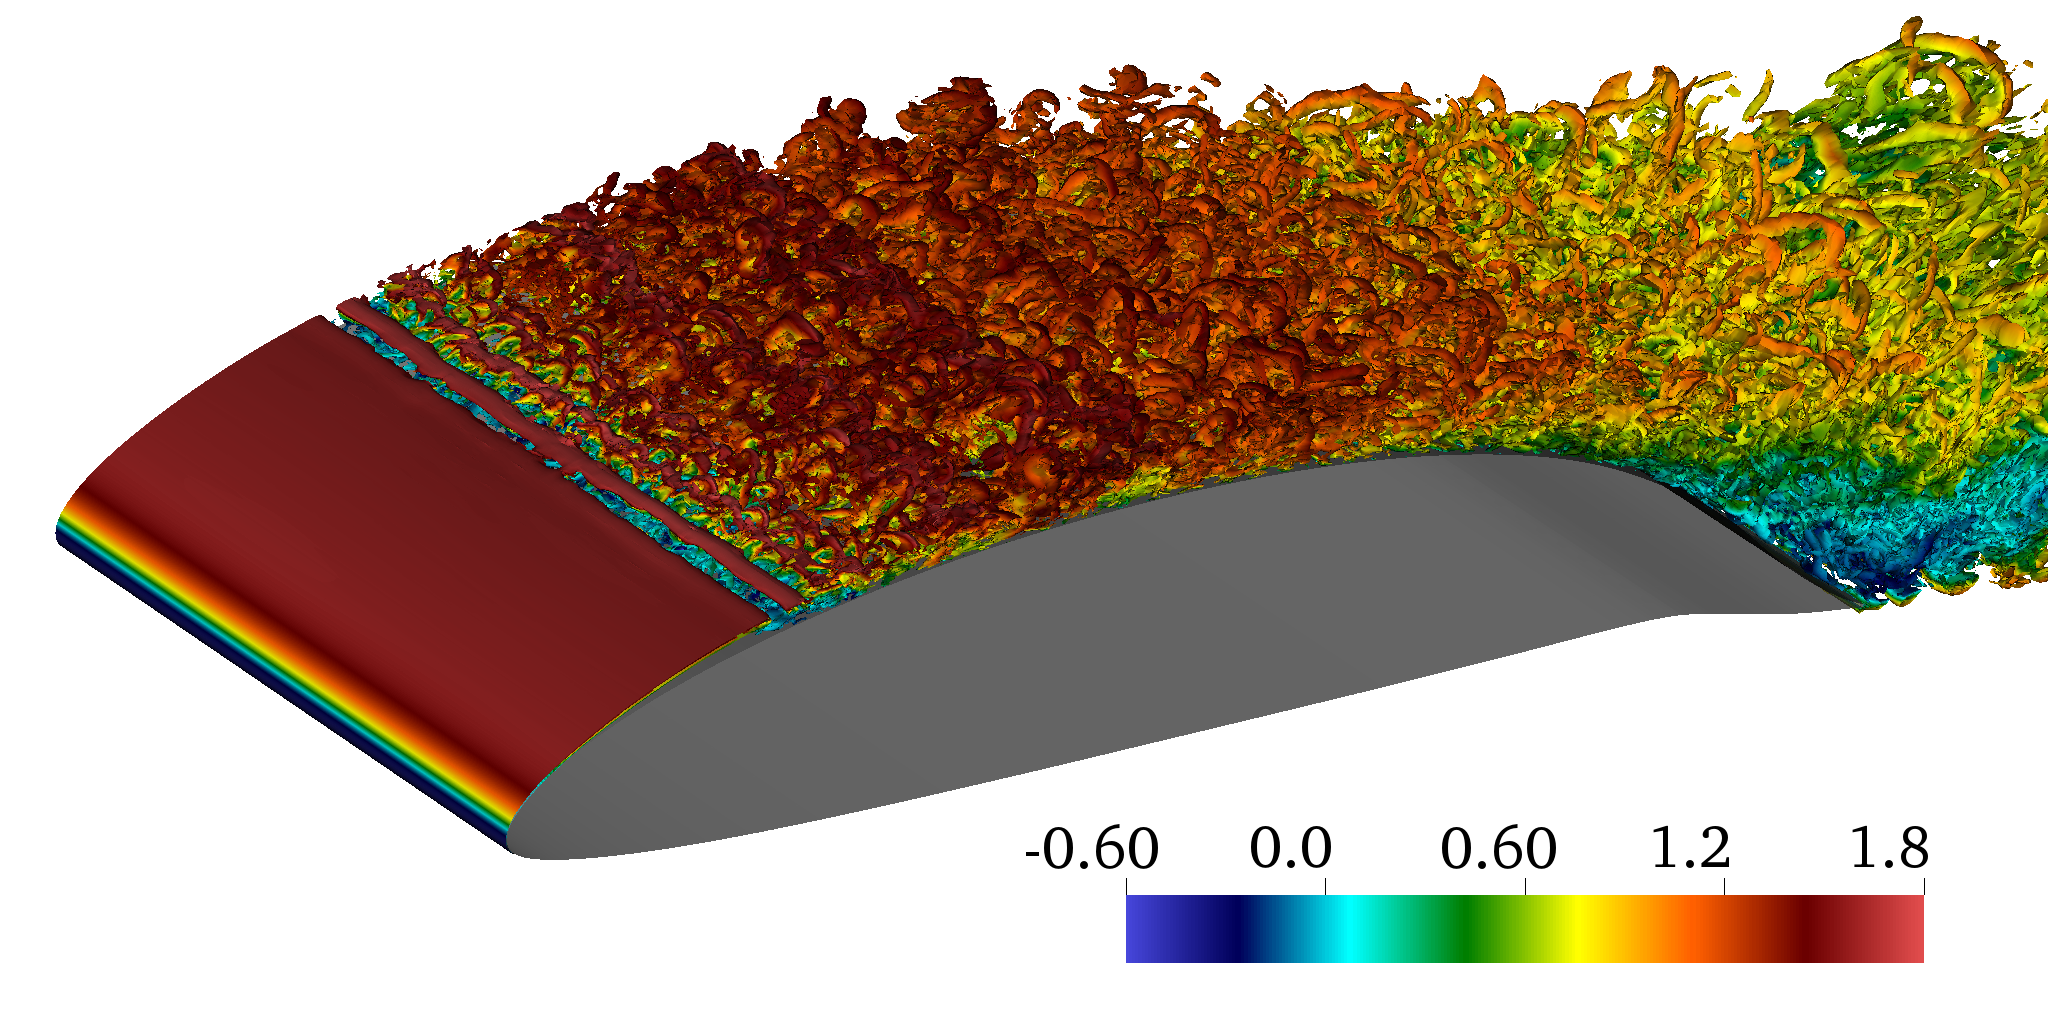
\includegraphics[width=1\textwidth]{re100k_static80_0001}
		\caption{$\alpha=8.0^{\circ}$}
		\label{fig:aoa80_iso}
	\end{subfigure}
	\caption{Isocontours of instantaneous $\lambda_{2}$ structures observed for two different (stationary) angles of attack.}
	\label{fig:isocontour_aoa}
\end{figure}

Simulations with a stationary airfoil were performed to investigate the location of transition without pitching motion. The simulations were performed for $Re_{c}=100,000$ at two different angles of attack ($\alpha=6.7^{\circ}$ and $\alpha=8.0^{\circ}$). As observed in figure~\ref{fig:isocontour_aoa}, the iso-contours of coherent structures, identified by negative $\lambda_{2}$ method \citep{jeong95}, show a substantial change in transition location for a small $\Delta\alpha=1.3^{\circ}$. For $\alpha=6.7^{\circ}$ the strong pressure gradient effects near the trailing edge cause transition at $x/c\approx0.7$. While for $\alpha=8.0^{\circ}$, a leading-edge laminar separation bubble forms, causing flow transition much closer to the leading edge at $x/c\approx0.2$. Such a leading-edge laminar separation bubble is not observed for the $\alpha=6.7^{\circ}$ case. The results are consistent with the trends obtained from XFOIL calculations, showing a large variation in the transition point within a small $\alpha$ change (figure~\ref{fig:xfoil_cm}).
%%%%%%%%%%%%%%%%%%%%%%%%%%%%%%%%%%%%%%%%%%%%%%%%%%%%%%%%%%%%%%%%%%%%%%
\subsection{Unsteady boundary layer characteristics}

Once the static characteristics of the airfoil are obtained, the dynamic effects on the boundary layer are investigated by pitching the airfoil about a mean angle $\alpha_{0}=6.7^{\circ}$ with an amplitude of $\Delta\alpha=1.3^{\circ}$. The reduced frequency of oscillation is $k=0.5$ and the pitch axis is located at $(x_{0},y_{0})=(0.35,0.034)$. The reduced frequency is defined as $k=\Omega b/U_{0}$, where $\Omega$ is the angular frequency of oscillation, $b$ is the semi-chord length and $U_{0}$ is the free-stream velocity. The motion of the airfoil is prescribed by equation~\ref{eqn:alpha_rule}. The pitching motion corresponds to an oscillation time period of $T_{osc}=2\pi$.
\begin{equation}
	\alpha = \alpha_{0} + \Delta\alpha\sin(\Omega t).
	\label{eqn:alpha_rule}
\end{equation}
The time variation of the coefficient of lift ($C_{L}$) is shown in figure~\ref{fig:cl-time-alpha}. The initial phase of pitching motion is carried out using a lower resolution (polynomial order $N=5$) to simulate the initial transient period of the flow at a lower computational cost. The polynomial order is then smoothly raised to $N=11$ before the fourth pitch cycle. Due to the fairly large separation at the trailing edge, effects of transition movement and turbulence, successive pitch cycles are not expected to have identical behavior, however some of qualitatively repeating trends can be observed. The behavior of the lift coefficient shows a chaotic but qualitatively repeating pattern where the lift coefficient shows a smooth increase during the pitch-up motion, with strong secondary effects occurring near the maxima of the pitch cycles. Similarly in the pitch-down phase the lift decreases smoothly with secondary effects again becoming important at the minima of the pitch-cycles.
\begin{figure}[h]
%	\begin{subfigure}[t]{0.5\textwidth}
		\centering
		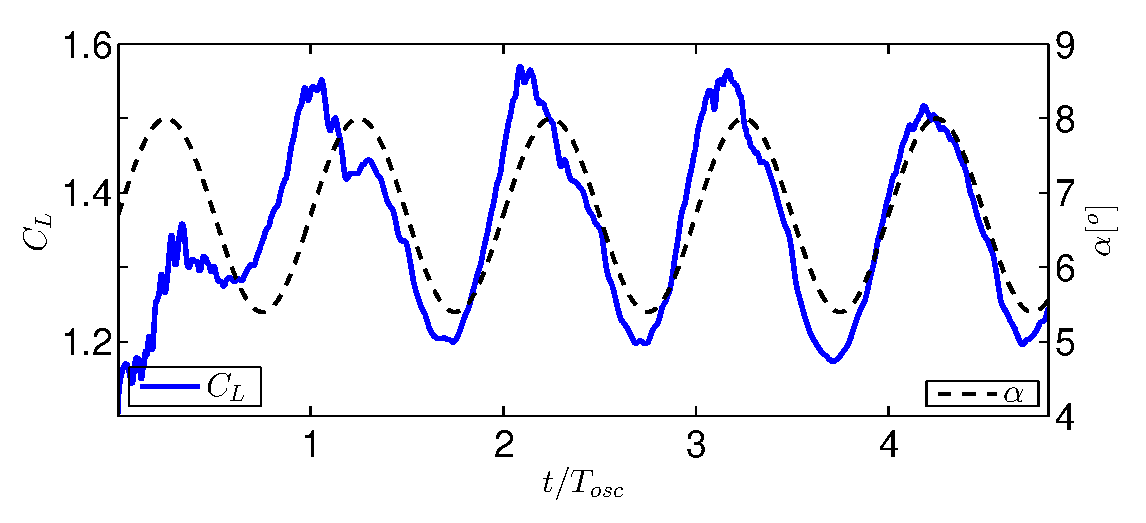
\includegraphics[width=0.9\textwidth]{cl-time-alpha}
%		\caption{Time variation}
		\caption{Coefficient of lift ($C_{L} \textcolor{blue}{-}$) and angle of attack $(\alpha \textcolor{black}{--})$ variation with time. $C_{L}$ is on the left axis while $\alpha$ is on the right axis.}
		\label{fig:cl-time-alpha}
%	\end{subfigure}
%	\begin{subfigure}[t]{0.45\textwidth}
%		\centering
%		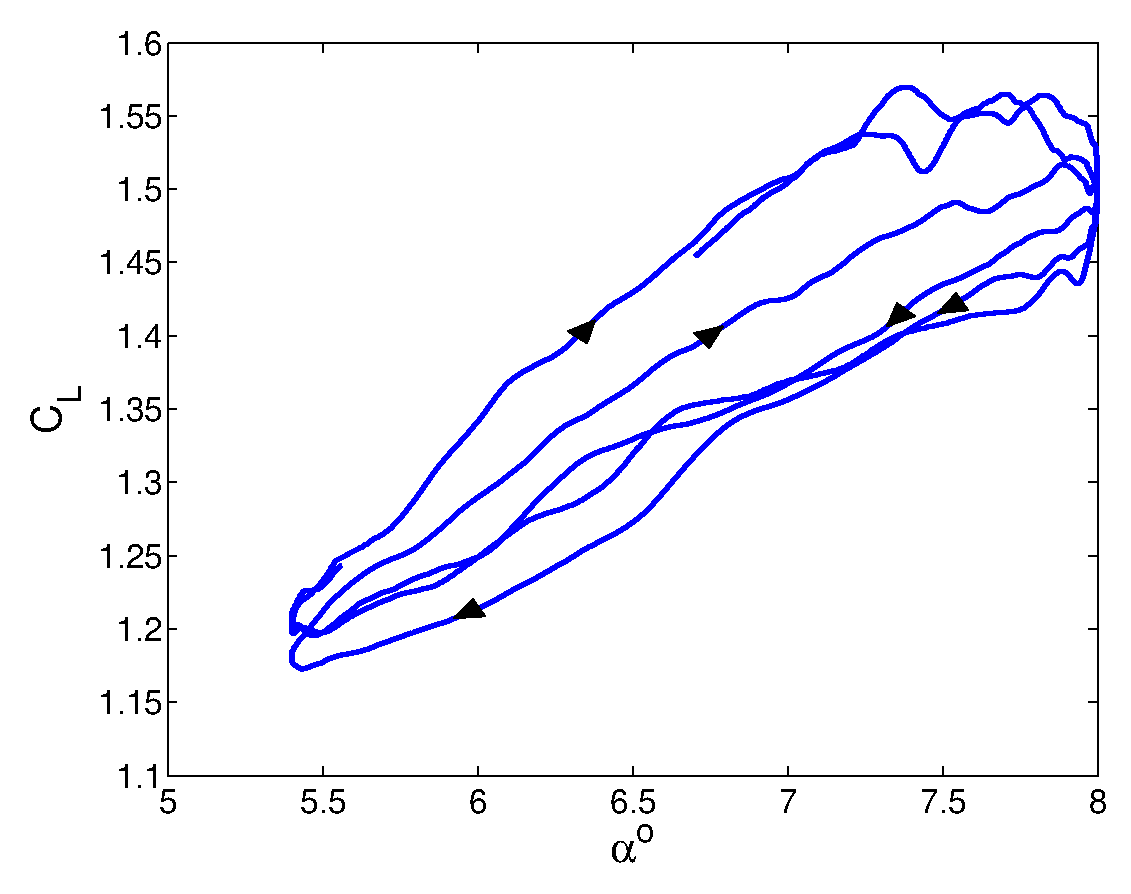
\includegraphics[width=1\textwidth]{cl-alpha}
%		\caption{Phase portrait}
%		\label{fig:cl-alpha}
%	\end{subfigure}
%	\caption{Coefficient of Lift ($C_{L} \textcolor{blue}{-}$) and angle of attack $(\alpha \textcolor{black}{--})$ variation with time (a) . $C_{L}$ is on the left axes while $\alpha$ is on the right axes. Phase portrait of $C_{L}$ and $\alpha$ (b). The sense of motion in figure (b) is clockwise, as marked by the arrows.}
\end{figure}

In order to understand the time variation of the spatially developing boundary layer on the airfoil, we analyze the space-time evolution of the instantaneous spanwise averaged wall-shear stress. The space-time surface plot is shown in figure~\ref{fig:cf-time}, which spans the fourth and fifth pitch cycles. The color specifies the value of wall-shear stress on the suction side of the airfoil. Regions with color intensity strongly towards red are indicative of high shear and thus turbulent flow. The exception to the rule being the region close to the leading edge where the flow is laminar but a high shear region exists due to the extremely thin boundary layer close to the stagnation point. The same space-time surface is shown again as a binary colored surface plot in figure~\ref{fig:separation-time}, where black colored regions indicate negative wall-shear stress and hence separated flow, while the white region corresponds to locations with attached flow ($\tau_{w}>0$).
\begin{figure}[h]
	\centering
	\begin{subfigure}[t]{0.45\textwidth}
		\centering
		\includegraphics[width=1\textwidth, height=1.5\textwidth]{cf_time_surf100k}
		\caption{Wall-shear stress ($\tau_{w}$).}. 
		\label{fig:cf-time}
	\end{subfigure}
	\begin{subfigure}[t]{0.45\textwidth}
		\centering
		\includegraphics[width=1.\textwidth, height=1.5\textwidth]{cf_time_surf_grey100k}
		\caption{Separated regions (black).} 
		\label{fig:separation-time}
	\end{subfigure}
	\caption{Space-time plot for the wall-shear values ($\tau_{w}$) and separated flow regions. The values are obtained from the instantaneous flow averaged over the spanwise direction. Horizontal blue dashed lines in (b) represent the extrema of the angle of attack, while the red dashed lines represent phases corresponding to mean angle of attack.}
	\label{fig:space-time}
\end{figure}

It is obvious from the two plots in figure~\ref{fig:space-time}, that the developing boundary layer on the airfoil exhibits a dynamically rich response to small-amplitude pitch oscillations, with different key boundary layer characteristics controlling the dynamics of the flow in different phases of the pitch cycle. We identify some of the key boundary layer characteristics to paint an over-all picture of the dynamics. A persistent trailing edge separation can be identified in figure~\ref{fig:separation-time} beyond $x/c>0.8$. The trailing-edge separation does not exhibit reverse flow 100\% of the time, as can be seen from the white patches dispersed between largely black colored regions. An isolated separated region (distinct from the trailing edge separation) is observed at $x/c\approx0.6$ at times $t/T_{osc}\approx3$ and $t/T_{osc}\approx4$. This is identified as a trailing-edge LSB. This LSB is short lived in time, existing for slightly less than a quarter of the pitch-cycle. A large separated region near the leading edge is a leading-edge LSB, similar to the one seen in the steady case at $\alpha=8.0^{\circ}$. The separation bubble persists much longer in time, spanning nearly half a pitch cycle. Evident from figure~\ref{fig:cf-time} is that the transition point changes substantially throughout the pitch cycle. Interestingly, the flow over the airfoil differs significantly during the pitch-up and the pitch-down phases for the same angle of attack. For example, when the instantaneous angle of attack is at phase $\phi=0\ (t/T_{osc}=3,\ 4)$, which represents mean angle of attack but in the pitch-up phase, the flow over the airfoil is mostly laminar up to $x/c\approx0.7$. On the other hand, for a phase of $\phi=\pi\ (t/T_{osc}=3.5,\ 4.5)$, representing the airfoil at the mean angle of attack but in the pitch-down phase, the flow is almost entirely turbulent with the start of the turbulent region approximately at $x/c\approx0.25$.

\subsection{Transition location}

In the present work we focus on the variation of transition location throughout the pitch cycles. Since the flow case is unsteady, and the transition location does not remain fixed, a criteria based on the instantaneous state of the flow is needed to determine the transition location. To this end, we calculate flow statistics which are averaged in the homogeneous spanwise direction, and also averaged for a short duration ($\Delta t$) in time, which is considered as the instantaneous value for that quantity. Thus the instantaneous value of any statistical quantity $\overline{q}(x,y,t)$ can be evaluated as in equation~\ref{eqn:inst_q}:
\begin{align}
	\overline{q}(x,y,t) = \left(\frac{1}{z_{max}-z_{min}}\right)\left(\frac{1}{\Delta t}\right)\int_{t'=t}^{t'=t+\Delta t}\int_{z=z_{min}}^{z=z_{max}}q(x,y,z,t')\ dz\ dt'.
	\label{eqn:inst_q}
\end{align}
Here $(z_{max}-z_{min})$ is the spanwise extent of the computational domain. In order for such a quantity to be representative of the instantaneous state of the flow, the time duration of the averaging must be small. For the current case we use $\Delta t=4\times10^{-3}$, which amounts to $0.06\%$ of the oscillation time period during which the flow can be assumed to remain in the same state. Using this procedure we evaluate the fluctuating Reynolds stress, $\overline{u'v'}(x,y,t)$, in order to determine the instantaneous transition location. The first streamwise location (on the suction-side) where the fluctuating Reynolds stress becomes larger than a certain threshold is denoted as the transition point. 
In order to prescribe a suitable threshold, the maximum value of $|\overline{u'v'}|$ across the entire boundary layer is evaluated for all times. This maximum value does not exhibit large variations, remaining within the same order of magnitude for all times with its mean value being $|\overline{u'v'}|_{max}\approx0.05$. The threshold for determining transition is set to $5\%$ of this value. The transition point is thus the first point where $|\overline{u'v'}|>0.0025$. Since we use an ad-hoc criterion for transition location, this is cross-checked by evaluating the variance of the spanwise velocity fluctuations $\overline{w'w'}$, and following an identical procedure as described above. In this case the transition criterion is prescribed as $|\overline{w'w'}|>0.005$ since the peak spanwise fluctuation intensities are found to be nearly twice the peak Reynolds stress $|\overline{u'v'}|$. Physically, growing spanwise velocity fluctuations indicate the onset of three-dimensionality in the boundary layer, which are associated with secondary instabilities. While the thresholds specified may be considered ad-hoc, the qualitative picture of transition movement is not very sensitive to small changes in the threshold. Changing the thresholds by a factor of 2 still produces the same qualitative trends (not shown). Figure~\ref{fig:space-time_tr} shows the calculated transition locations superposed on the wall-shear stress and separation space-time plots. The calculated transition locations are consistent with the picture of wall-shear stress with transition marginally preceding regions of turbulent flow. Moreover, the time variation of transition point determined by two different physical quantities agree very well with each other. Thus we consider the quantities as a good representations of instantaneous flow characteristics.
\begin{figure}[h]
	\centering
	\begin{subfigure}[t]{0.45\textwidth}
		\centering
		\caption{}. 
		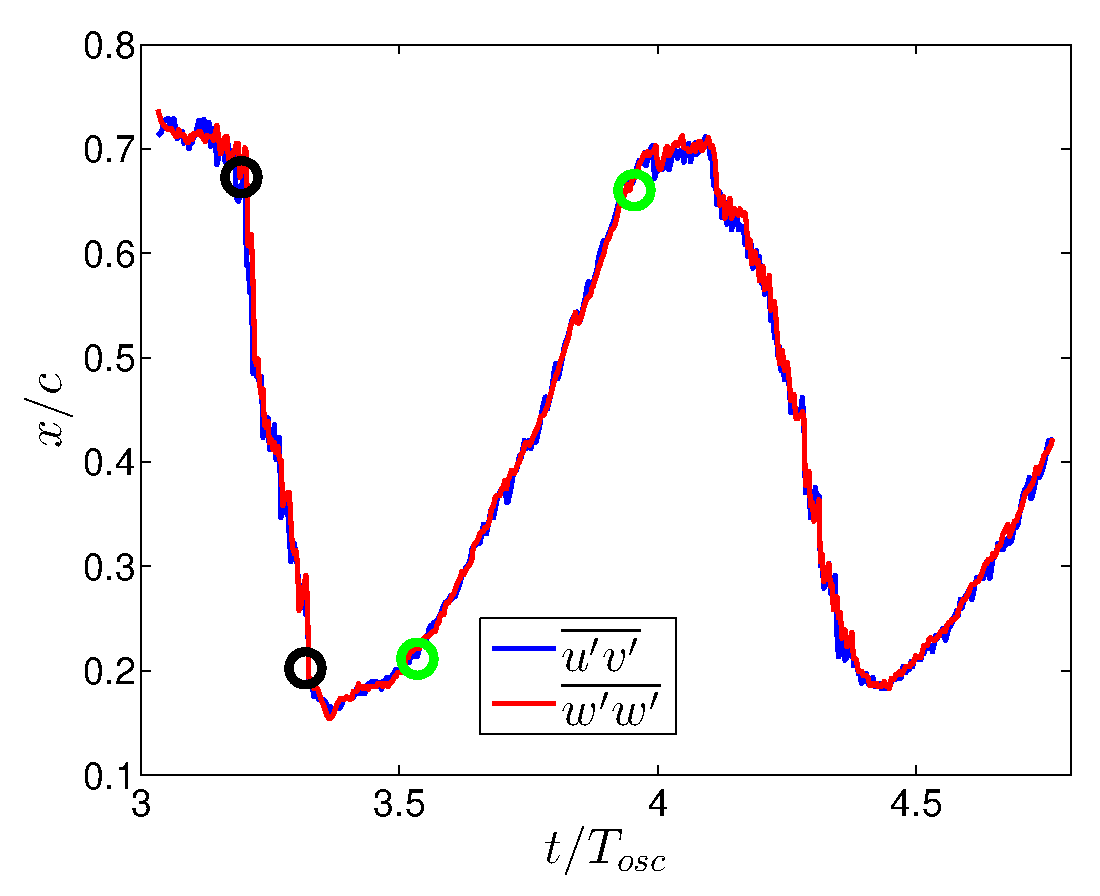
\includegraphics[width=1\textwidth]{transition_time}
		\label{fig:transition_time}
	\end{subfigure}
	\begin{subfigure}[t]{0.45\textwidth}
		\centering
		\caption{} 		
		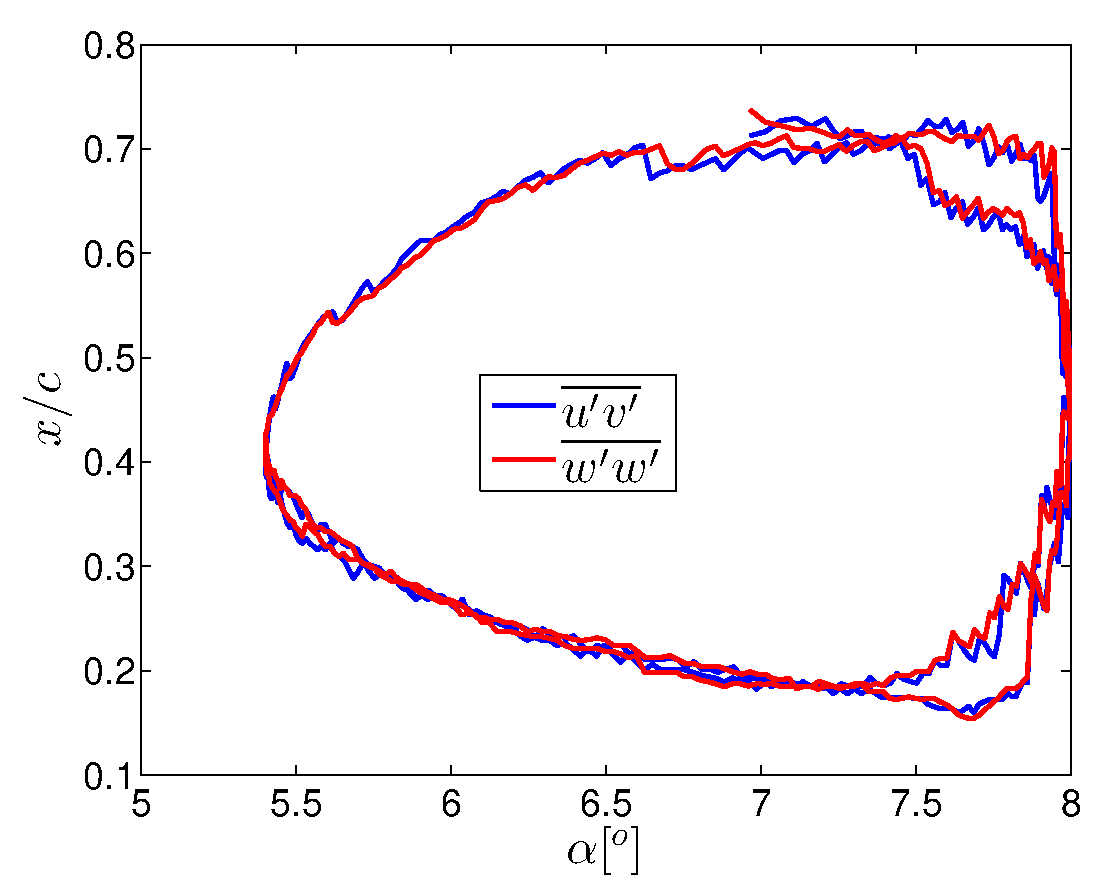
\includegraphics[width=1\textwidth]{transition_alpha}
		\label{fig:transition_alpha}
	\end{subfigure}
	\caption{Time variation (a) and phase portrait with $\alpha$ (b) of transition location evaluated using the criteria for $|\overline{u'v'}|$ and $|\overline{w'w'}|$. The circles mark the points used to approximate the upstream (black circles) and downstream (green circles) velocities of the transition point.}
	\label{fig:transition}
\end{figure}

\begin{figure}[h]
	\centering
	\begin{subfigure}[t]{0.46\textwidth}
		\centering
		\includegraphics[width=1\textwidth, height=1.5\textwidth]{cf_time_surf100k_tr}
		\caption{Wall-shear stress ($\tau_{w}$).}. 
		\label{fig:cf-time_tr}
	\end{subfigure}
	\begin{subfigure}[t]{0.45\textwidth}
		\centering
		\includegraphics[width=0.97\textwidth, height=1.5\textwidth]{cf_time_surf_grey100k_tr}
		\caption{Separated regions (black).} 
		\label{fig:separation-time_tr}
	\end{subfigure}
	\caption{Transition locations indicated by the magenta line superposed on the space-time plots of wall-shear stress and separation.}
	\label{fig:space-time_tr}
\end{figure}

The superposed plots in figure~\ref{fig:space-time_tr} clearly indicate that the two LSBs play a dominating role in the flow dynamics and that transition location is governed by the characteristics of these LSBs. Figure~\ref{fig:transition_la2} (left) shows the iso-contours of instantaneous vortical structures, identified by the $\lambda_{2}$ method \citep{jeong95}, at four different times during the pitch-up cycle when the transition is moving upstream. This phase is marked by the appearance of a leading-edge LSB which grows in size. The top figure shows the flow state near the mean angle of attack ($t/T_{osc}=3.09$) during the pitch-up phase. The flow is mostly laminar across the airfoil with no structures observed prior to flow transition and the there is no leading-edge LSB. The high adverse pressure gradient near the trailing edge causes the laminar flow to easily separate, forming a LSB and flow transitions over this separated shear layer. Figure~\ref{fig:transition_la2} (left) from top to bottom shows the part of the oscillation cycle when transition is moving upstream at time instants of $t/T_{osc}=3.09,\ 3.2,\ 3.3$ and $3.47$. Note that pitch-up phase completes at $t/T_{osc}=3.25$ when the airfoil is at the highest angle of attack. Thus upstream movement of transition starts nearly at the end of the pitch-up phase and continues to move upstream even during the pitch-down cycle. The laminar separation bubble close to the trailing edge ceases to exist as transition moves upstream. At $t/T_{osc}=3.47$ the flow transition is seen to occur on the separated shear layer of the leading-edge LSB (bottom left in figure~\ref{fig:transition_la2}).

As the airfoil progresses through the pitch-down cycle the leading-edge LSB shrinks in size and the transition point then starts moving downstream, initiating the process of flow re-laminarization (figure~\ref{fig:transition_la2} right, top to bottom). The leading-edge LSB eventually disappears, although the transition point moves downstream of the LSB before it completely disappears. The flow over the airfoil is not completely re-laminarized even when the airfoil is at the lowest angle of attack and the re-laminarization process continues into the pitch-up phase. There is a marked asymmetry between the upstream and downstream movement of the transition point. An approximate velocity for both the upstream and downstream motion of the transition point is calculated across the points marked by circles in figure~\ref{fig:transition_time} which correspond to transition movement with near constant velocity. The velocity of upstream transition movement is calculated across the black circles and is equal to $V^{tr}_{u}=-0.60$ while the velocity of the downstream motion of transition is calculated across the green circles and is equal to $V^{tr}_{d}=0.17$. Thus the upstream spread of turbulent regions is much faster than flow re-laminarization. %At the moment it is unclear what causes the asymmetry between the upstream and downstream movement of transition, or if a symmetric movement can even be expected.

Specifying a velocity of transition movement implies that the transition location changes smoothly with time. This is true for the downstream movement of transition, however the final stages of the upstream movement appear to be more complex. Figure~\ref{fig:transition_complex} shows the instantaneous vortical structures at two time instants during the upstream movement phase. In the left figure a single connected region of turbulence can be observed which is preceded by a laminar region identified by the near absence of small vortical structures. On the right figure there are two distinct regions of turbulent flow separated by a patch of laminar flow. The emergence of two distinct turbulent regions signifies that transition occurs independently at different streamwise positions indicating that two and competing mechanisms exist for the growth of disturbances in the boundary layer and that their relative strength changes during the pitch cycle.

\begin{figure}
	\centering
	\begin{subfigure}[t]{0.48\textwidth}
		\centering
		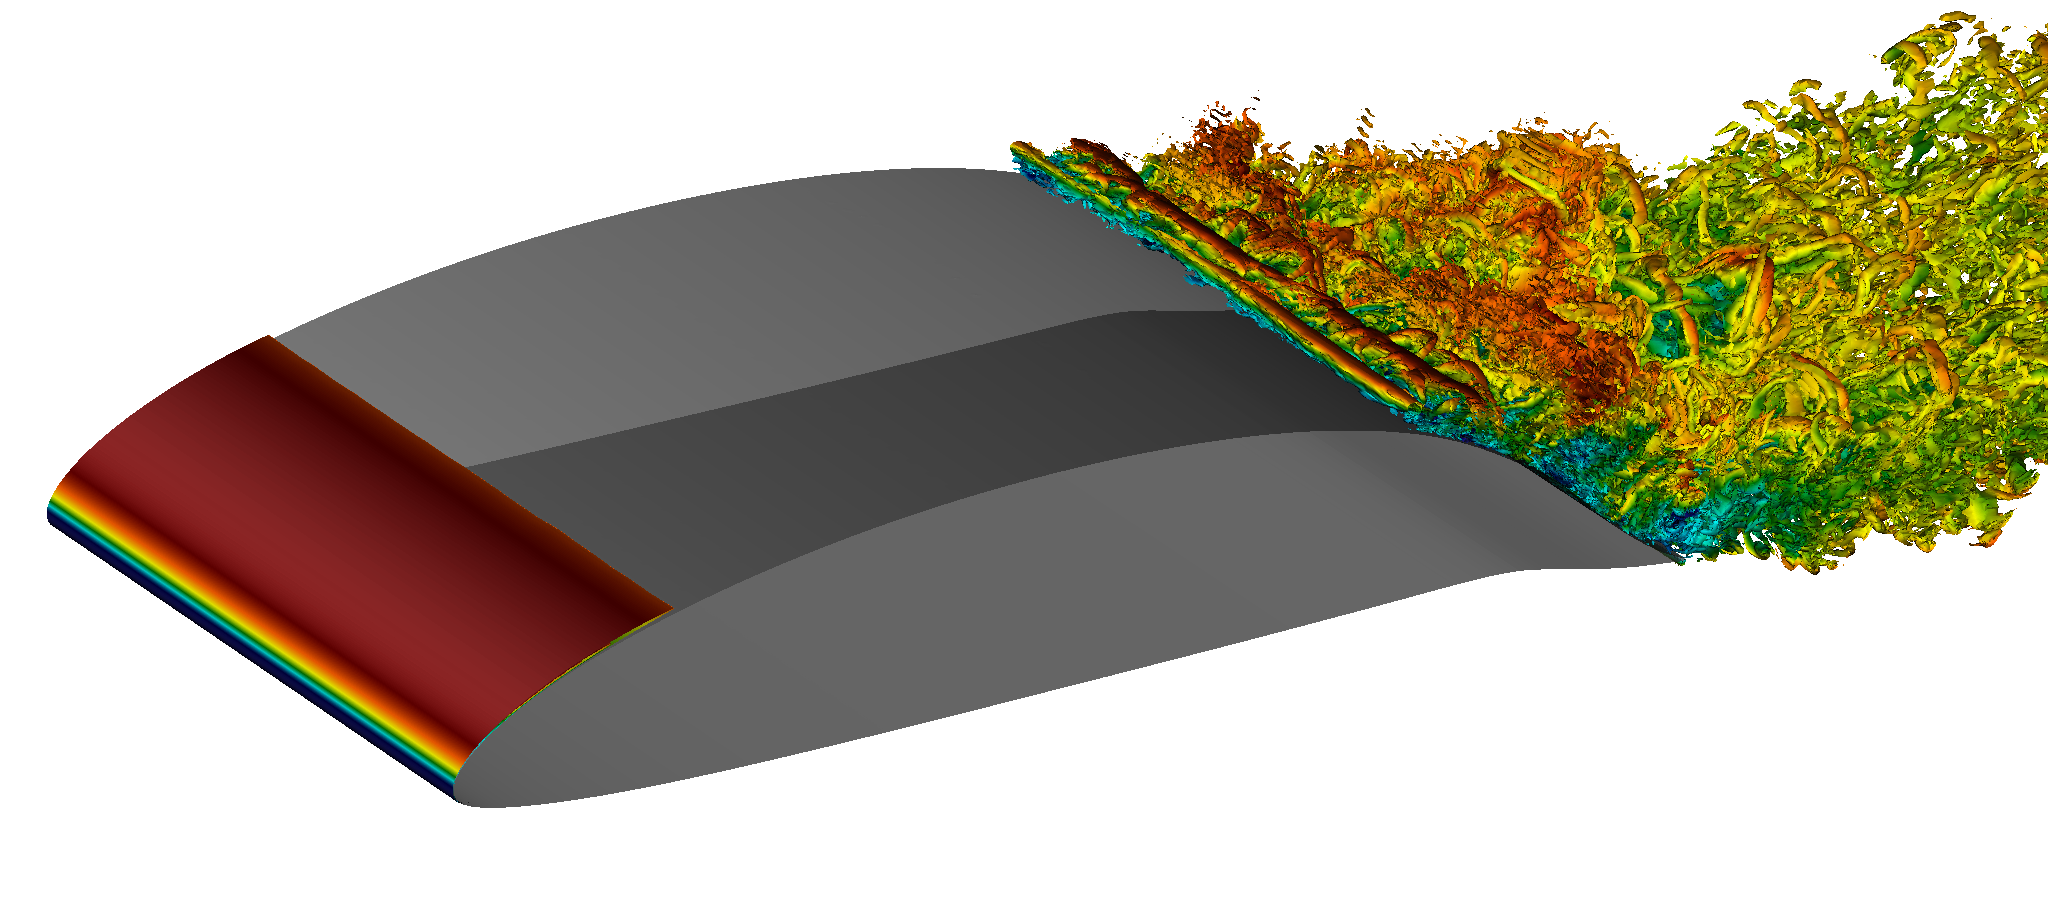
\includegraphics[width=1\textwidth]{pitchup0001.png}
		\label{fig:pitchup_1}
	\end{subfigure}
	\begin{subfigure}[t]{0.48\textwidth}
		\centering
		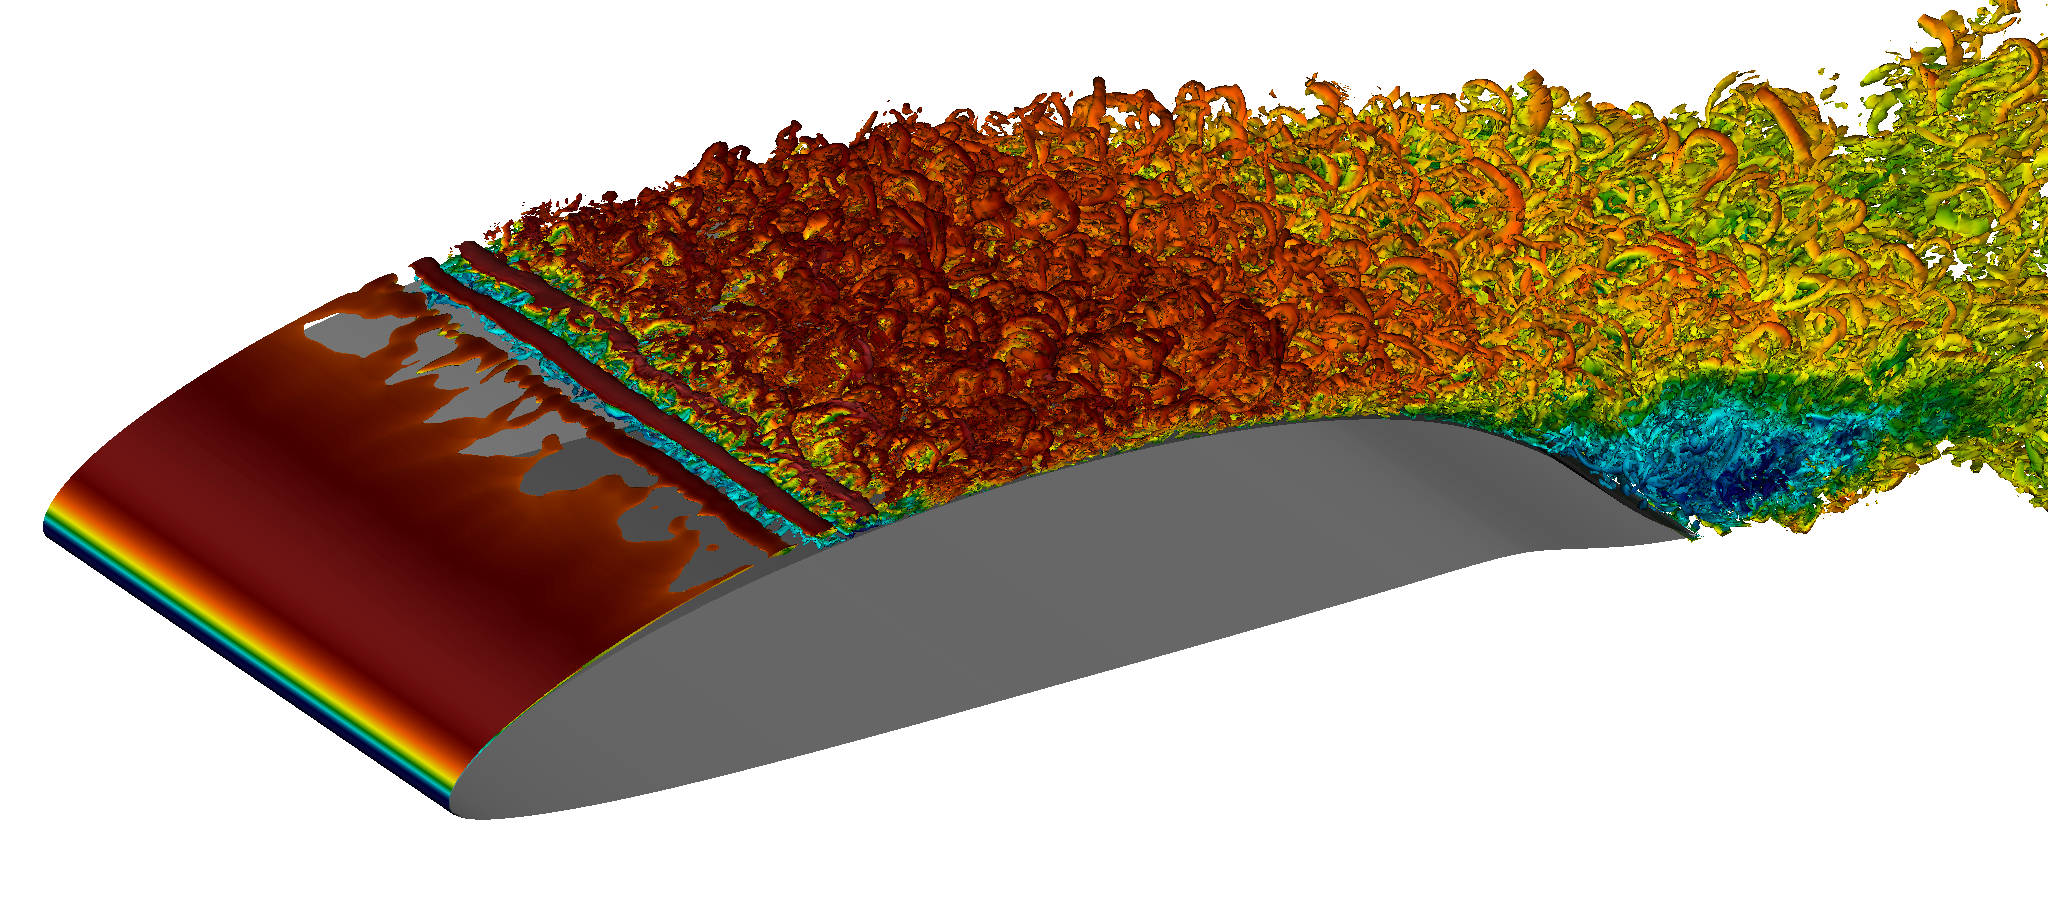
\includegraphics[width=1\textwidth]{relaminar0001.png}
		\label{fig:relaminar_1}
	\end{subfigure}
	\begin{subfigure}[t]{0.49\textwidth}
		\centering
		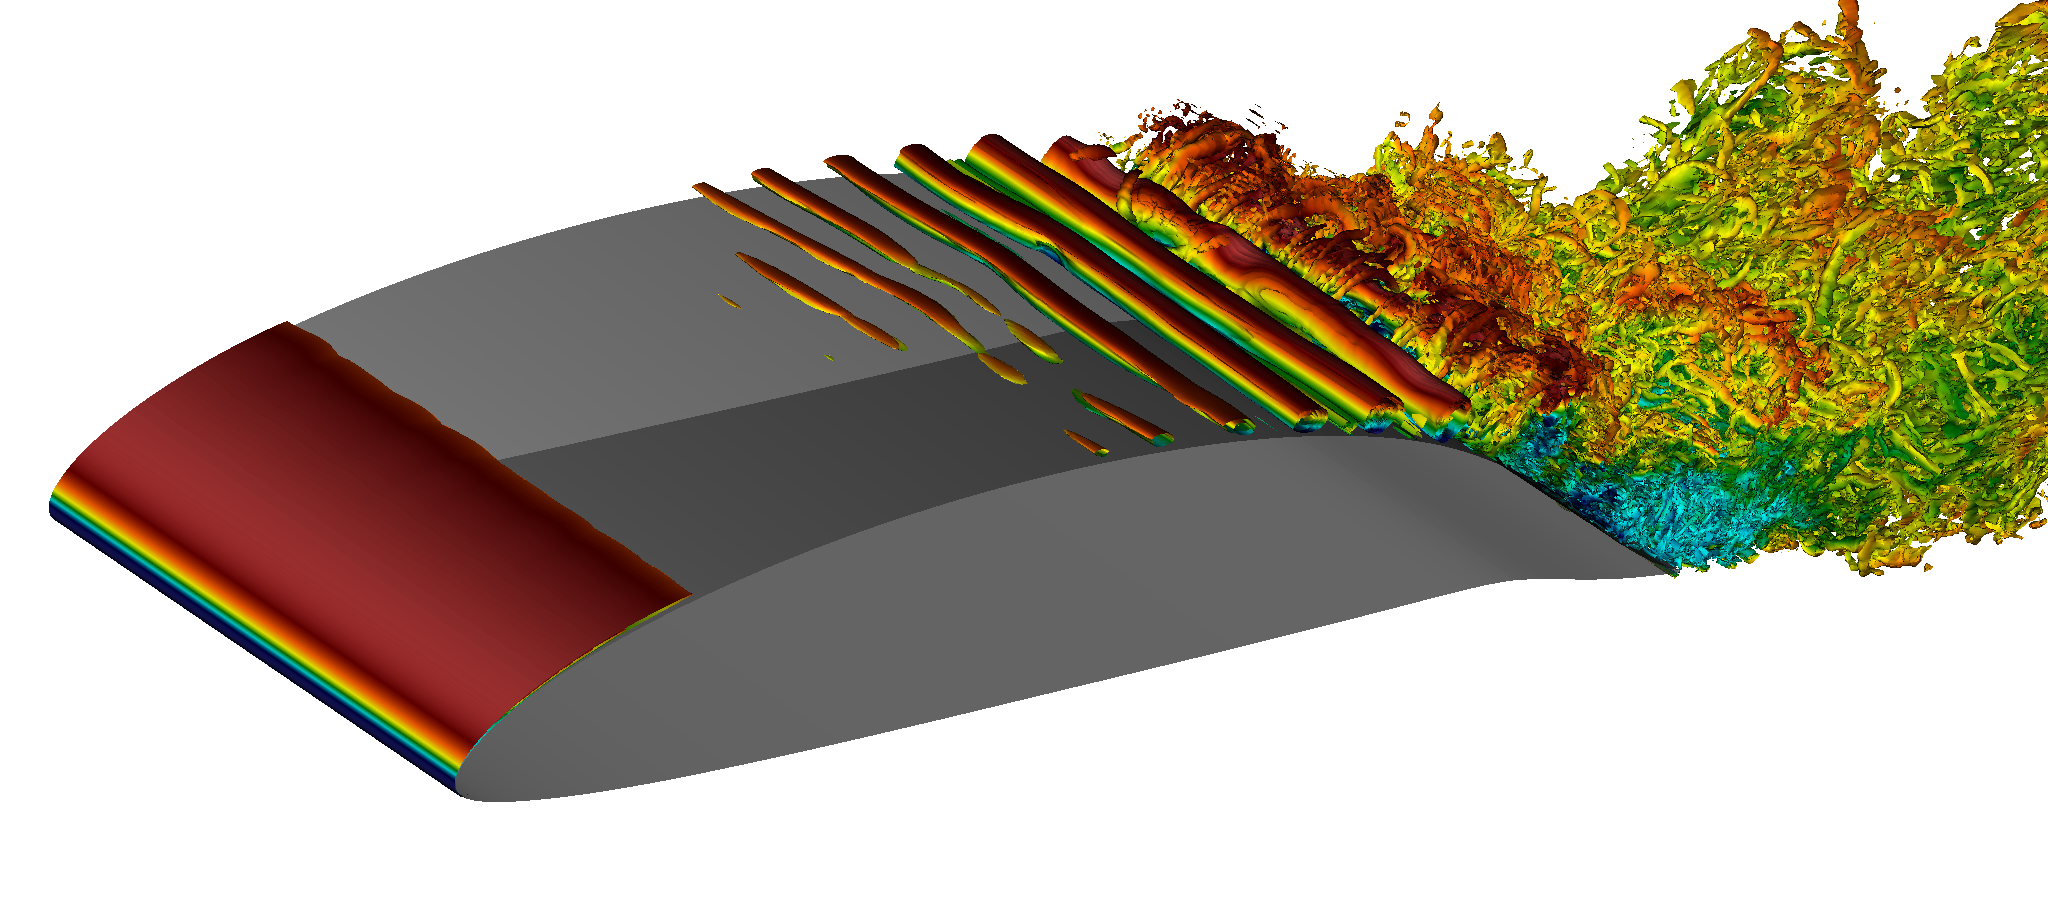
\includegraphics[width=1\textwidth]{pitchup0002.png}
		\label{fig:pitchup_2}
	\end{subfigure}
	\begin{subfigure}[t]{0.49\textwidth}
		\centering
		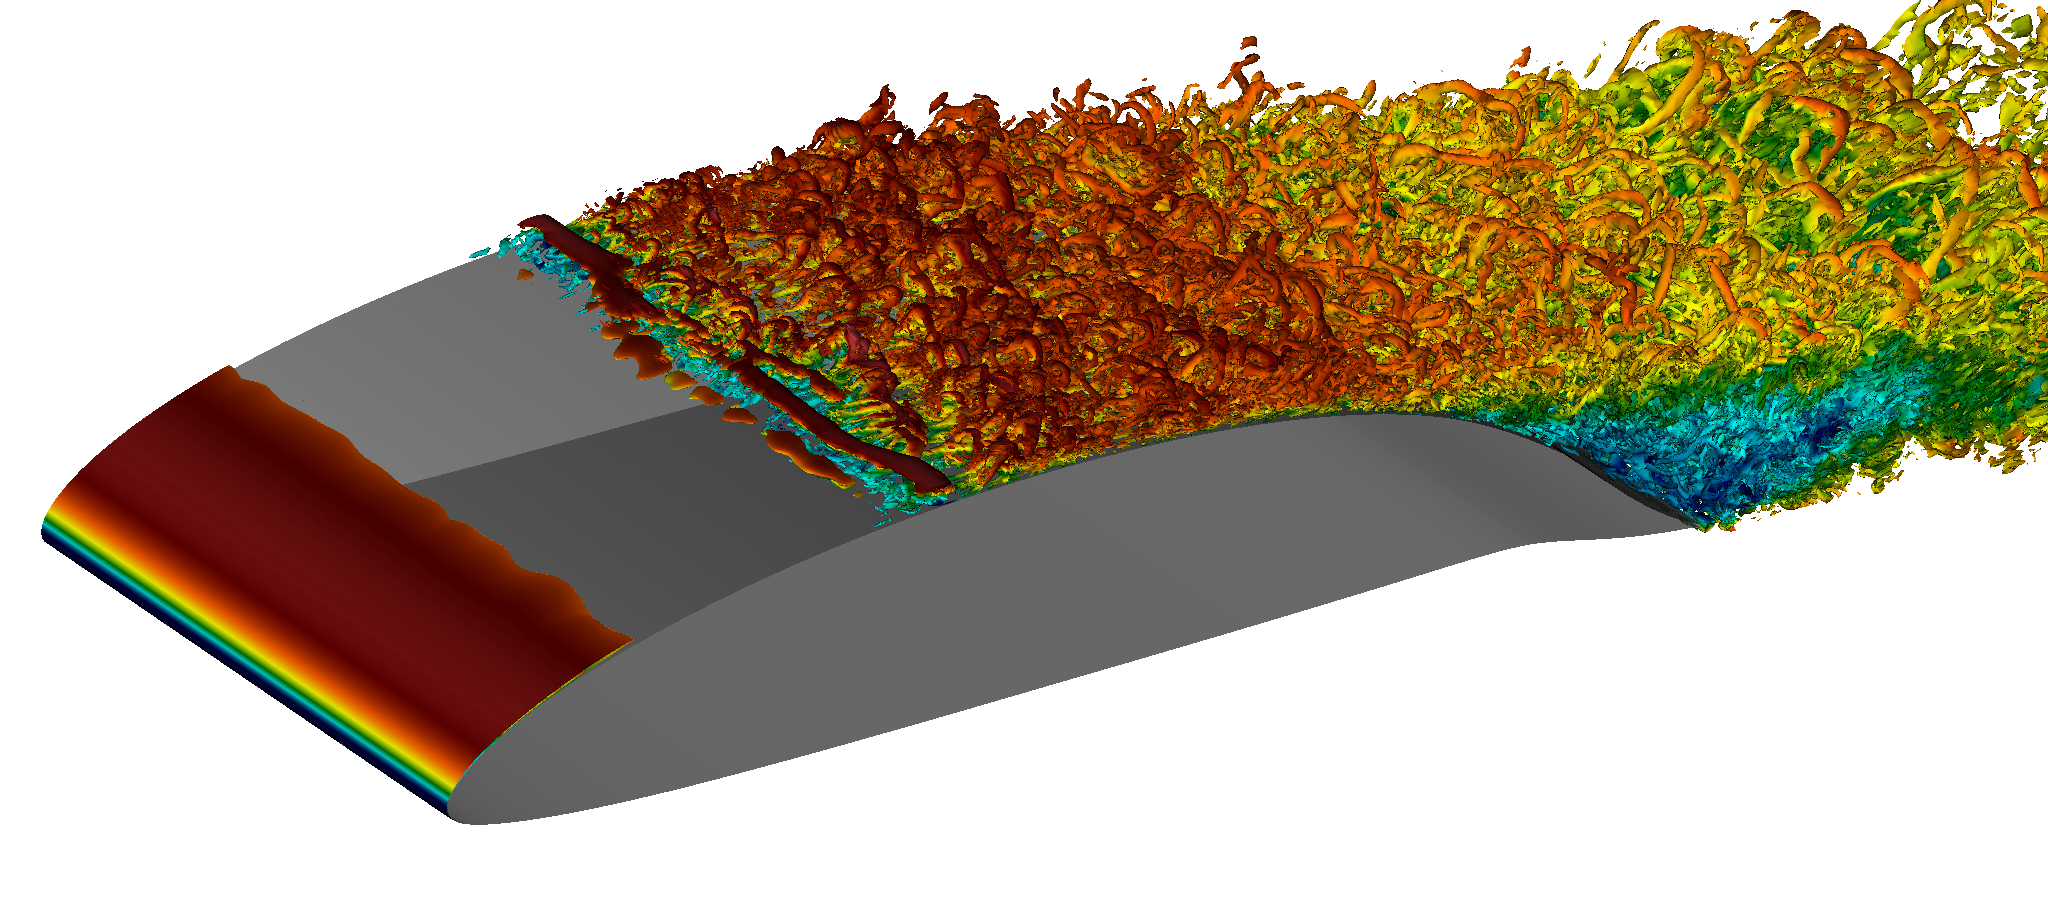
\includegraphics[width=1\textwidth]{relaminar0002.png}
		\label{fig:relaminar_2}
	\end{subfigure}
	\begin{subfigure}[t]{0.49\textwidth}
		\centering
		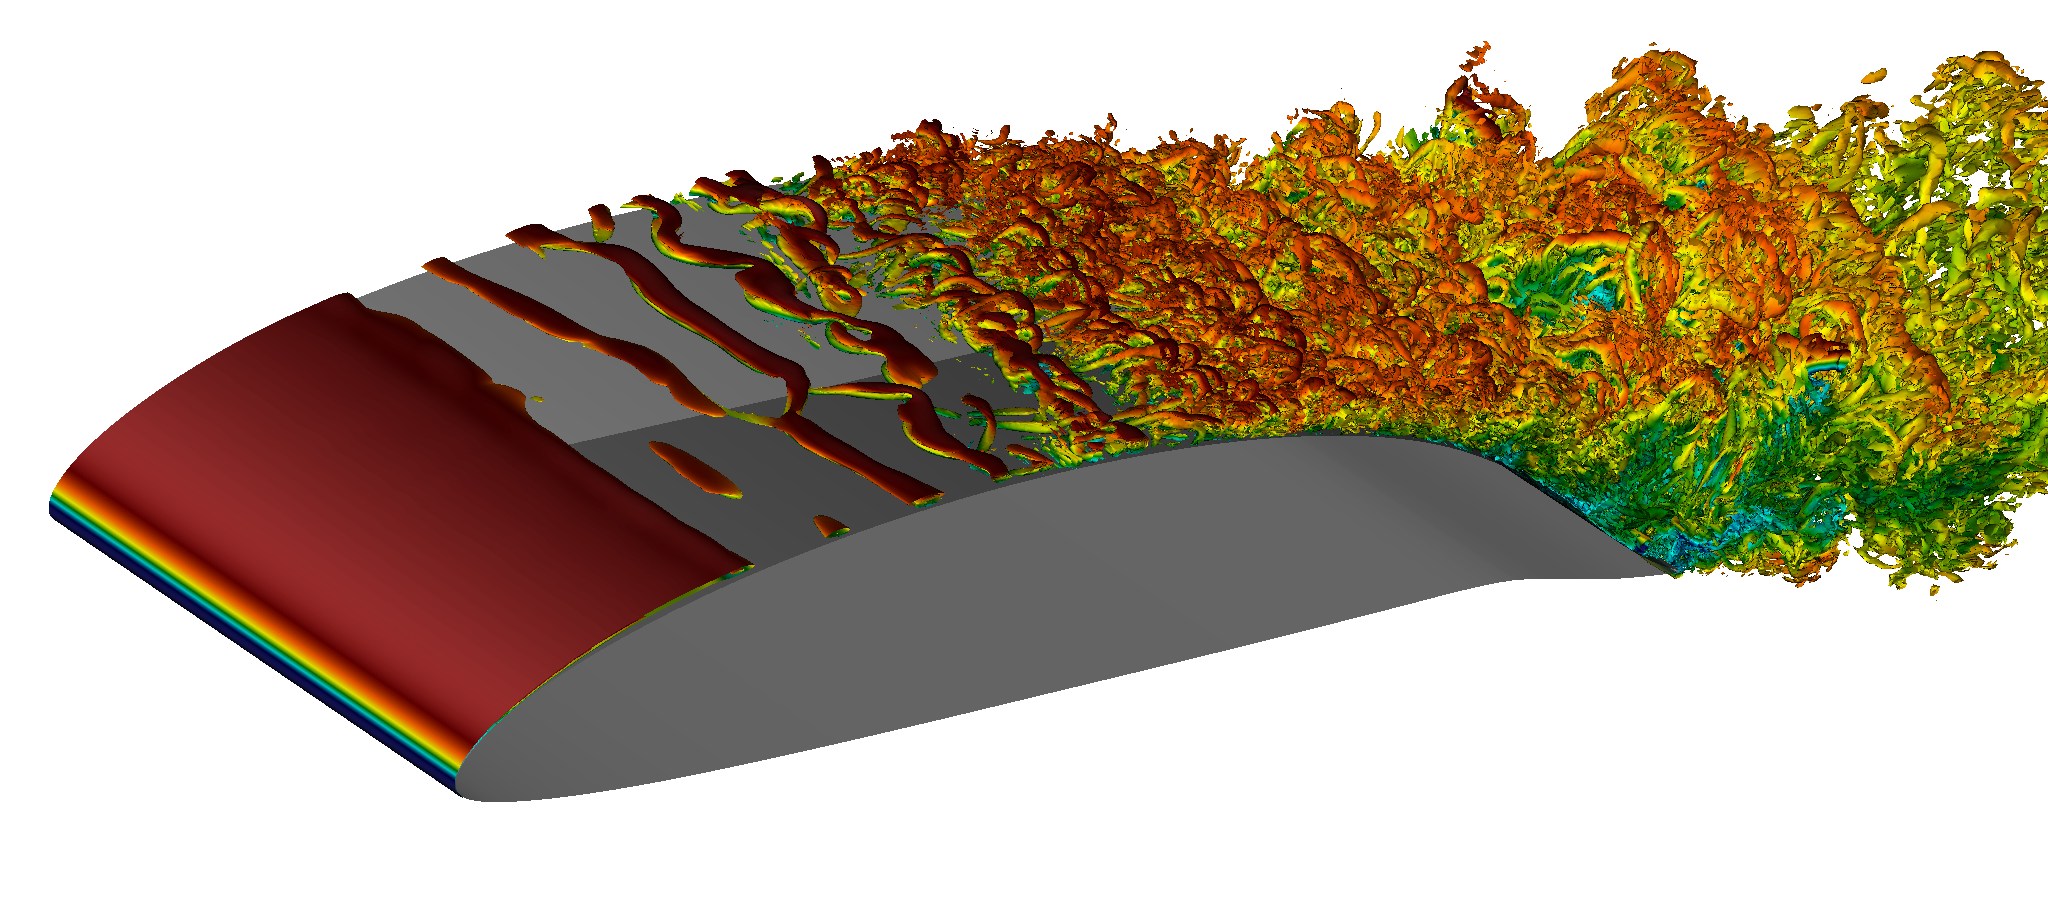
\includegraphics[width=1\textwidth]{pitchup0003.png}
		\label{fig:pitchup_3}
	\end{subfigure}
	\begin{subfigure}[t]{0.49\textwidth}
		\centering
		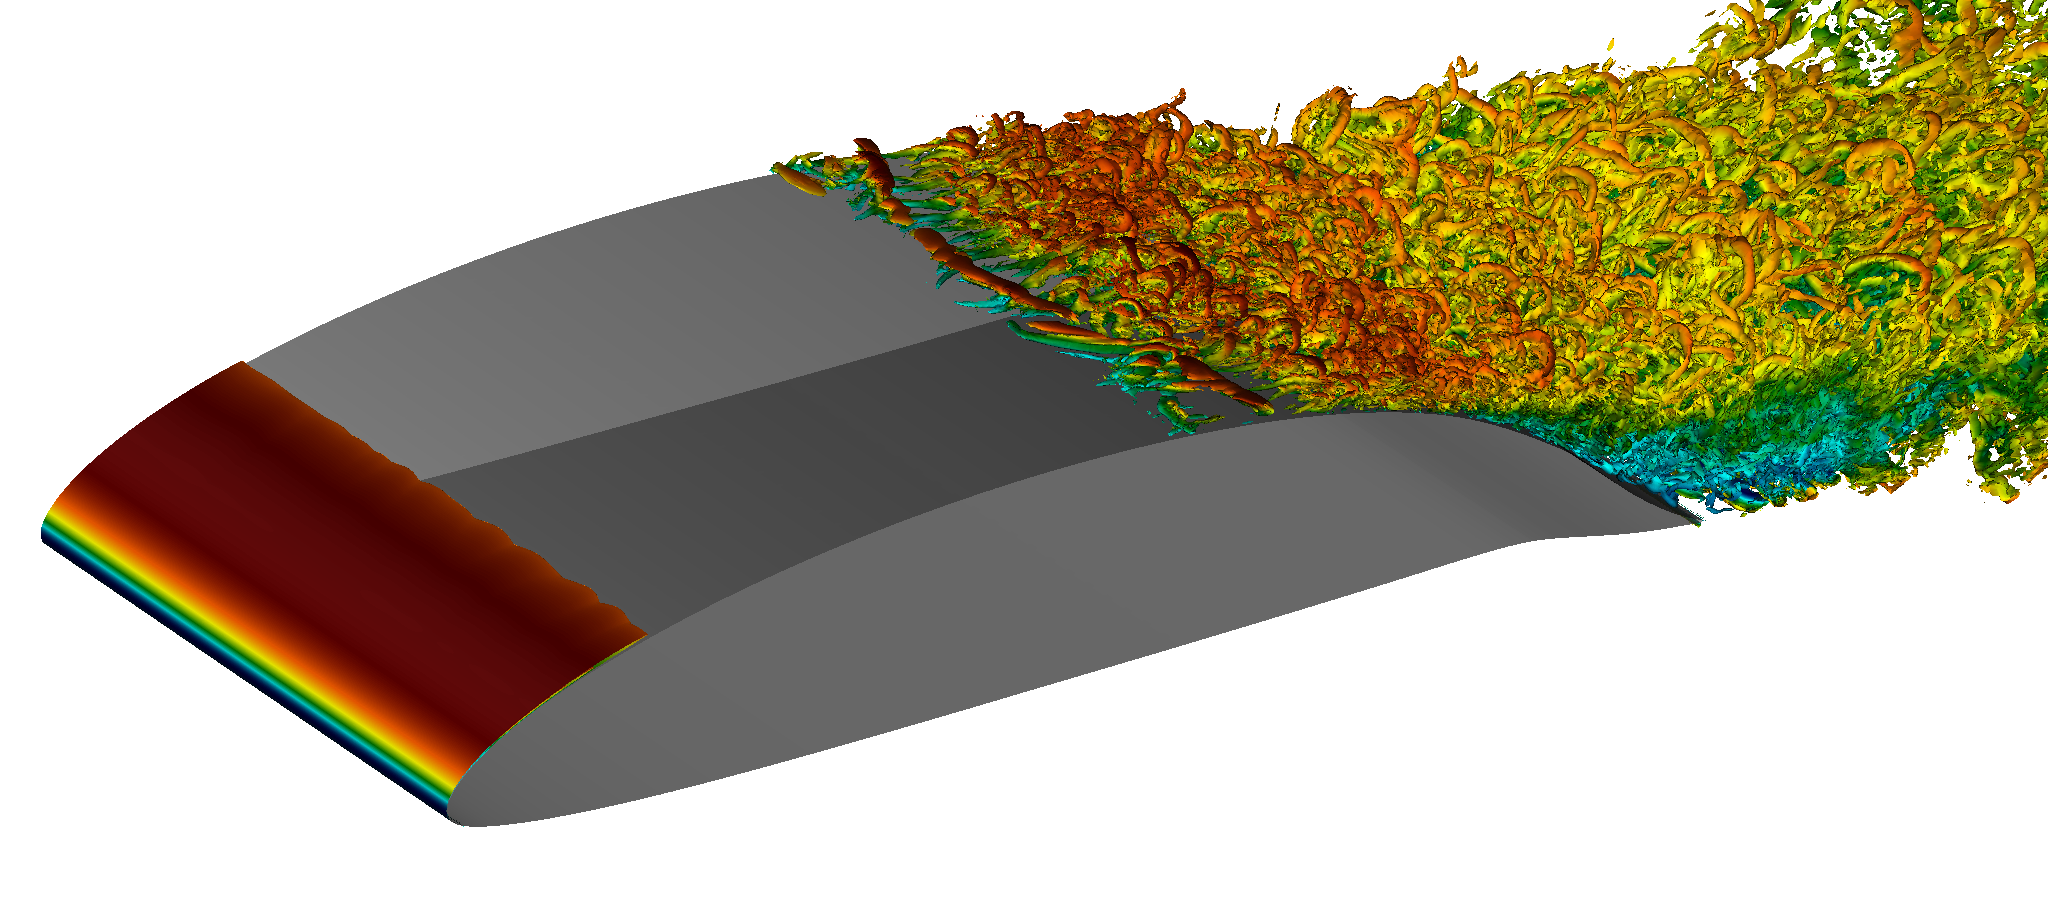
\includegraphics[width=1\textwidth]{relaminar0003.png}
		\label{fig:relaminar_3}
	\end{subfigure}
	\begin{subfigure}[t]{0.49\textwidth}
		\centering
		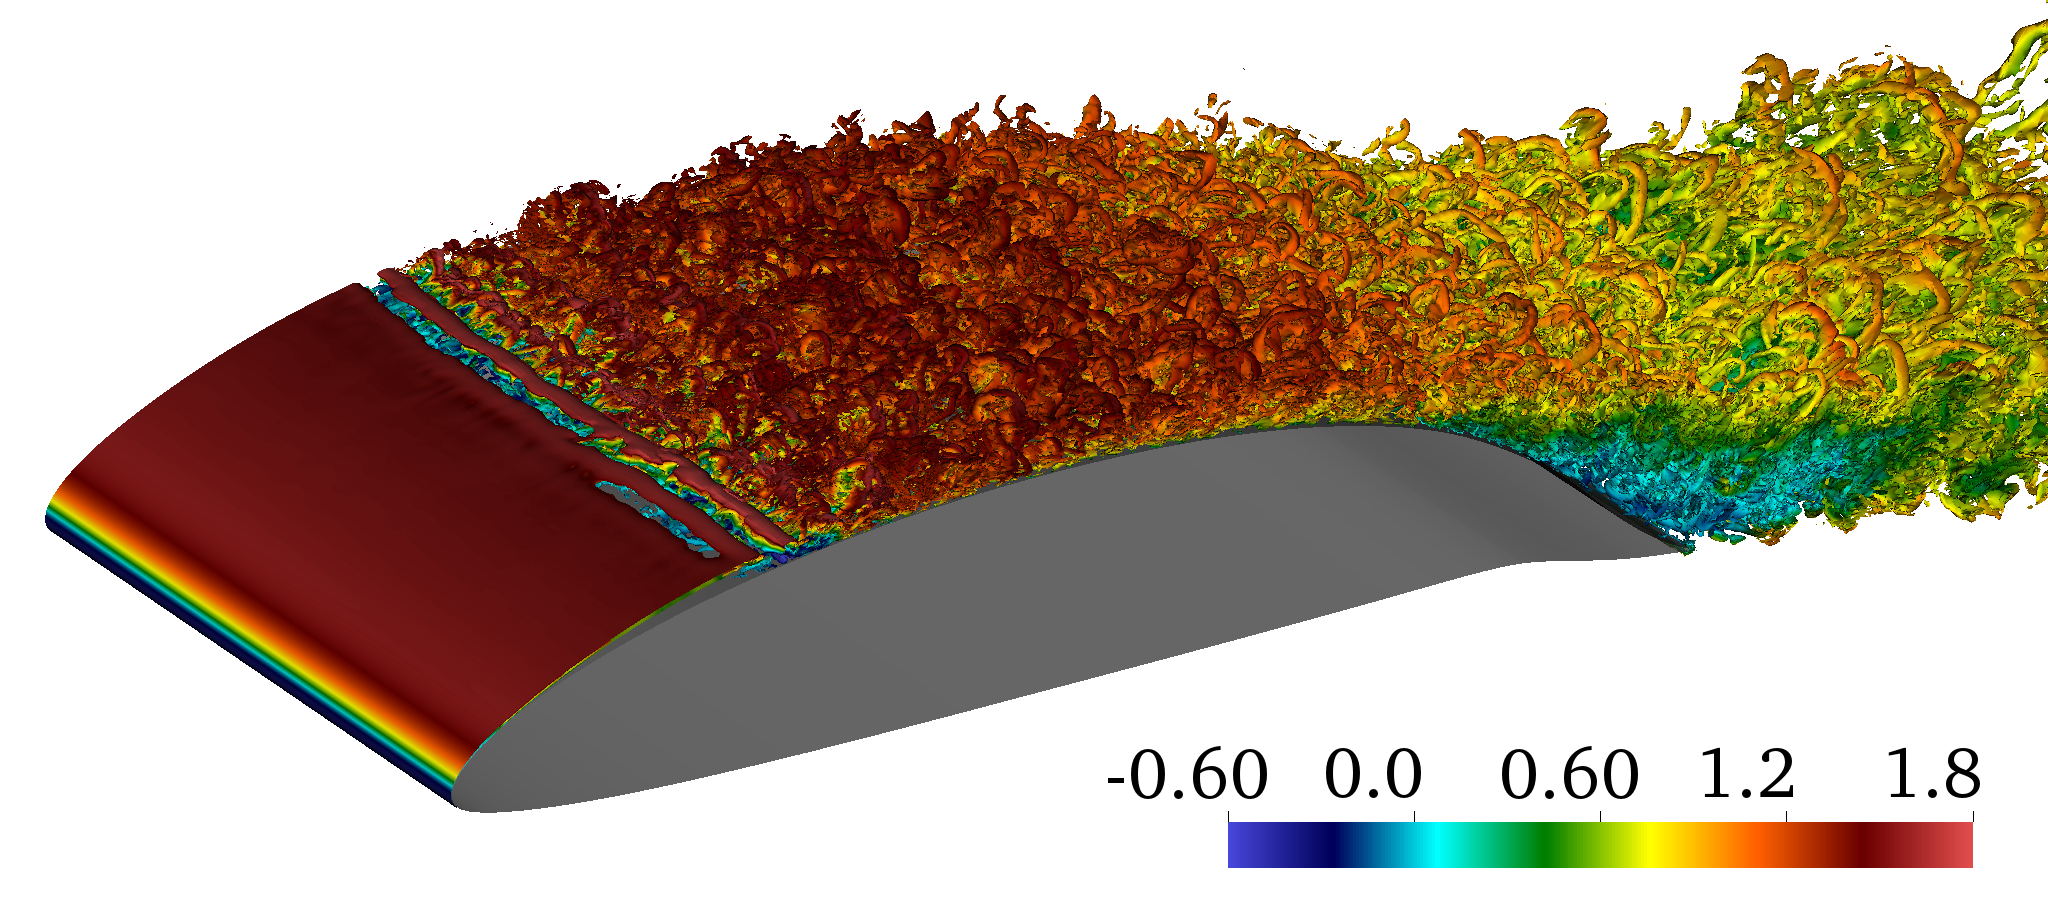
\includegraphics[width=1\textwidth]{pitchup0005.png}
		\label{fig:pitchup_4}
	\end{subfigure}
	\begin{subfigure}[t]{0.49\textwidth}
		\centering
		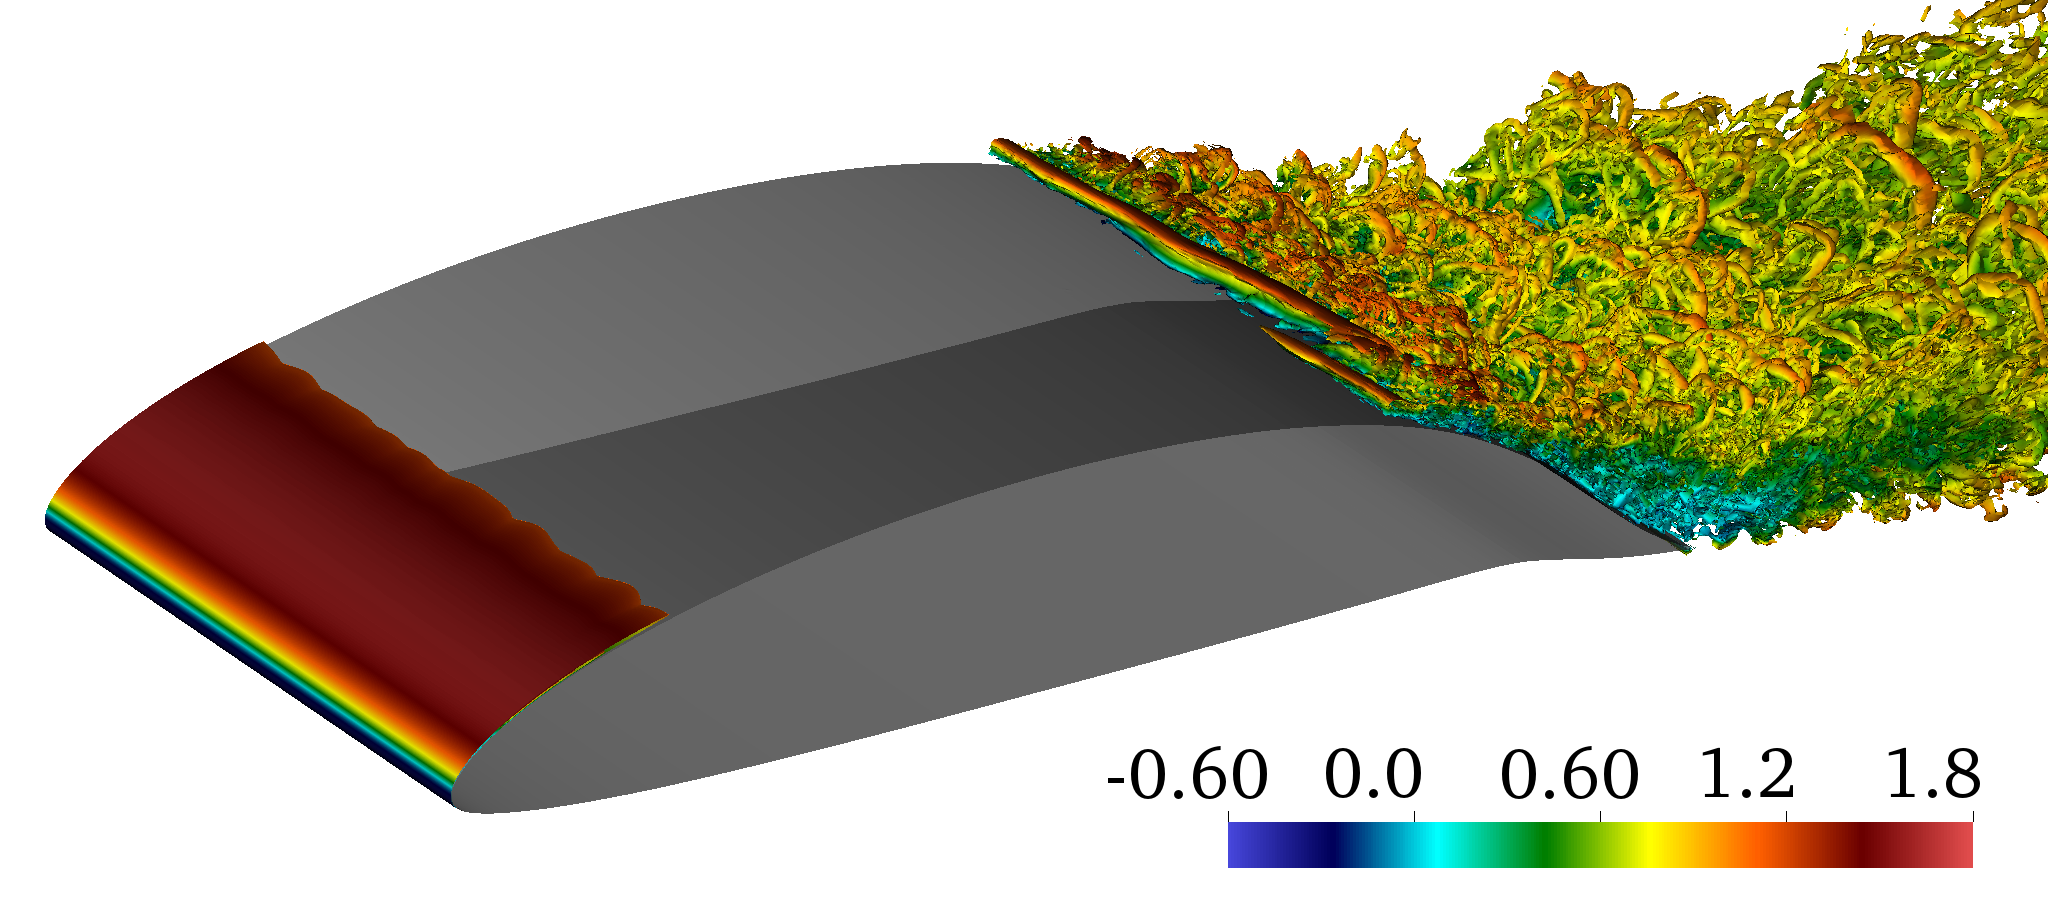
\includegraphics[width=1\textwidth]{relaminar0005.png}
		\label{fig:relaminar_4}
	\end{subfigure}	
	\caption{Visualization of instantaneous $\lambda_{2}$ structures at different phases of the pitch cycle. The figures on the left are during the phase of the pitch cycle when the transition is moving upstream. From top to bottom the time-stamps of the instantaneous snapshots correspond to a normalized flow time of $t/T_{osc}=3.09,\ 3.2,\ 3.3,\ 3.47$. On the right the instantaneous snapshot correspond to the re-laminarization phase as transition moves downstream. The time-stamps from top to bottom on the right correspond to $t/T_{osc}=3.55,\ 3.63,\ 3.82,\ 4.01$}
%	This corresponds to t=19.4015, 20.1655, 20.6975, 21.8295 during the pitchup motion.
%	This corresponds to t=22.3655, 22.8335, 24.0175, 25.2255 during the pitchup motion.	
	\label{fig:transition_la2}
\end{figure}


\begin{figure}
	\centering
	\begin{subfigure}[t]{0.48\textwidth}
		\centering
		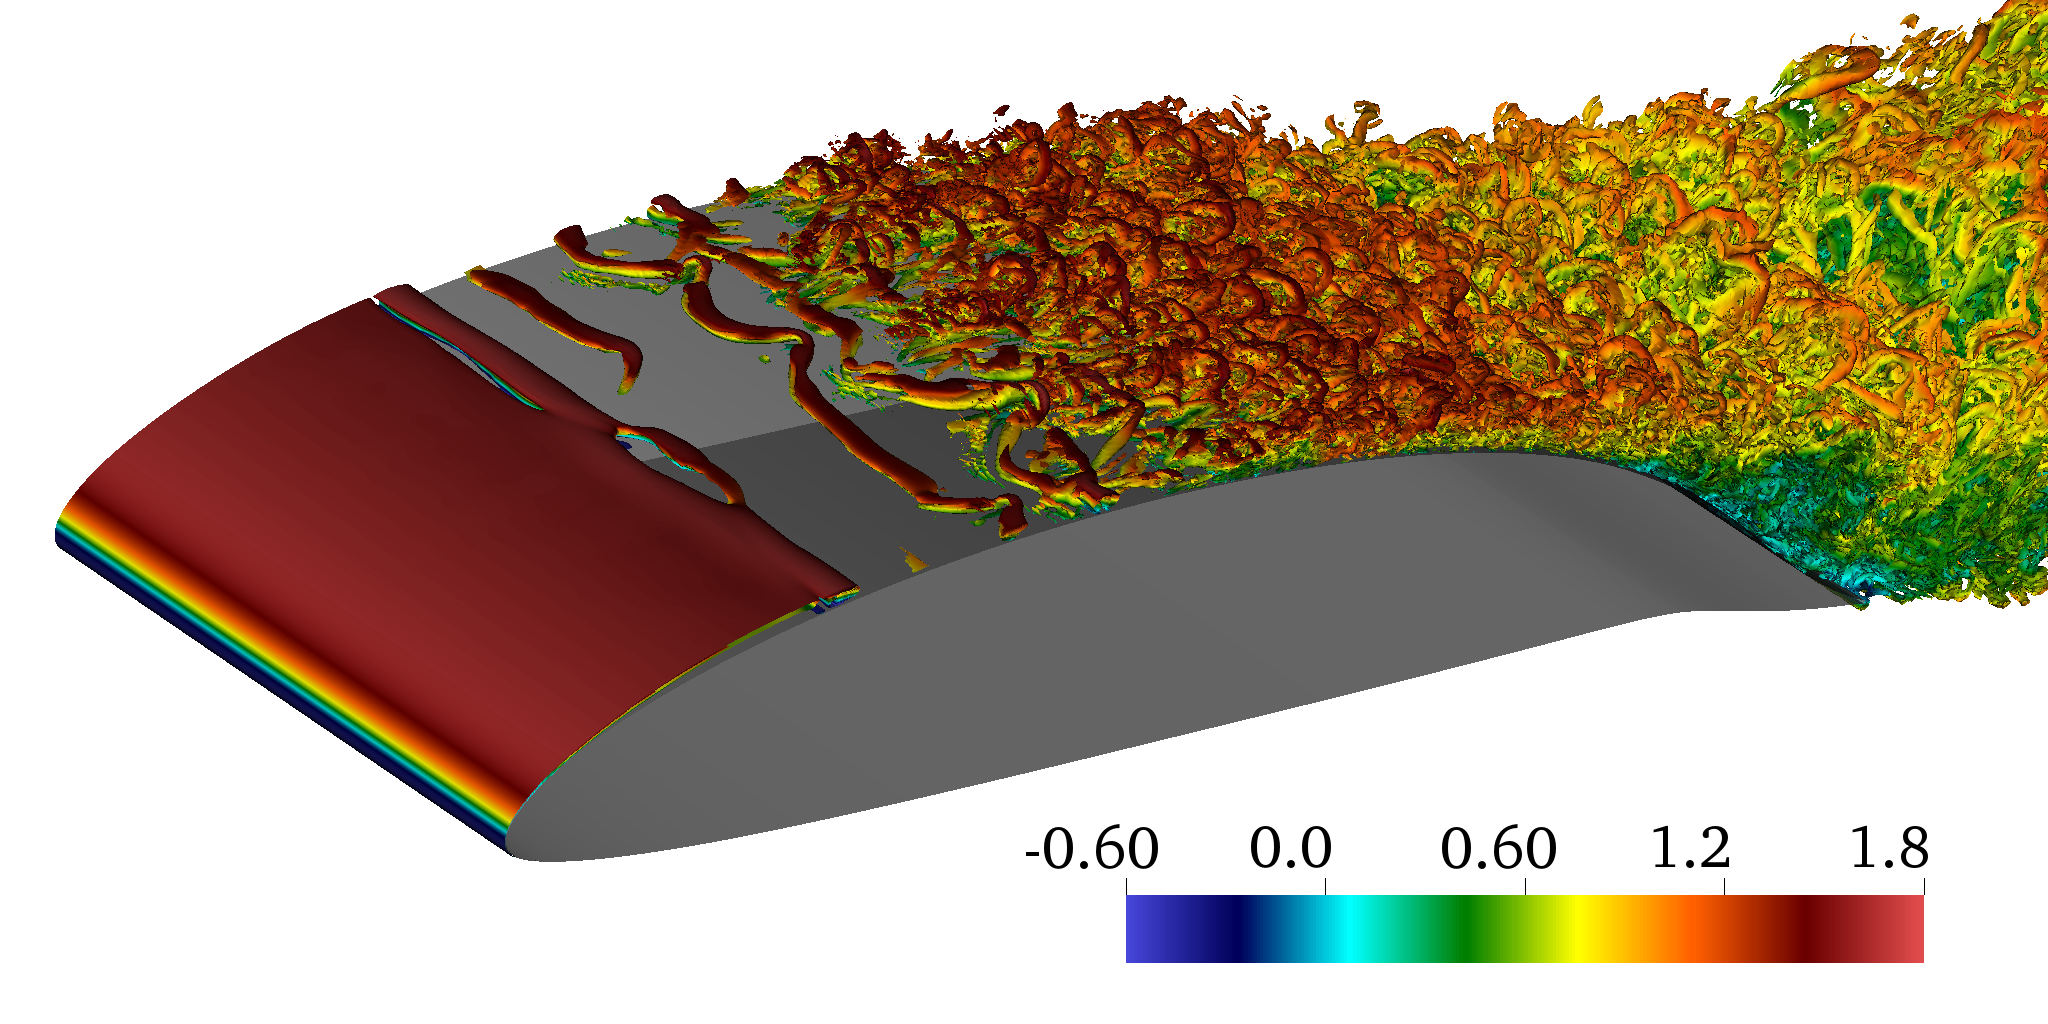
\includegraphics[width=1\textwidth]{pitch_re100k0260}
		\label{fig:upstream_1}
	\end{subfigure}
	\begin{subfigure}[t]{0.48\textwidth}
		\centering
		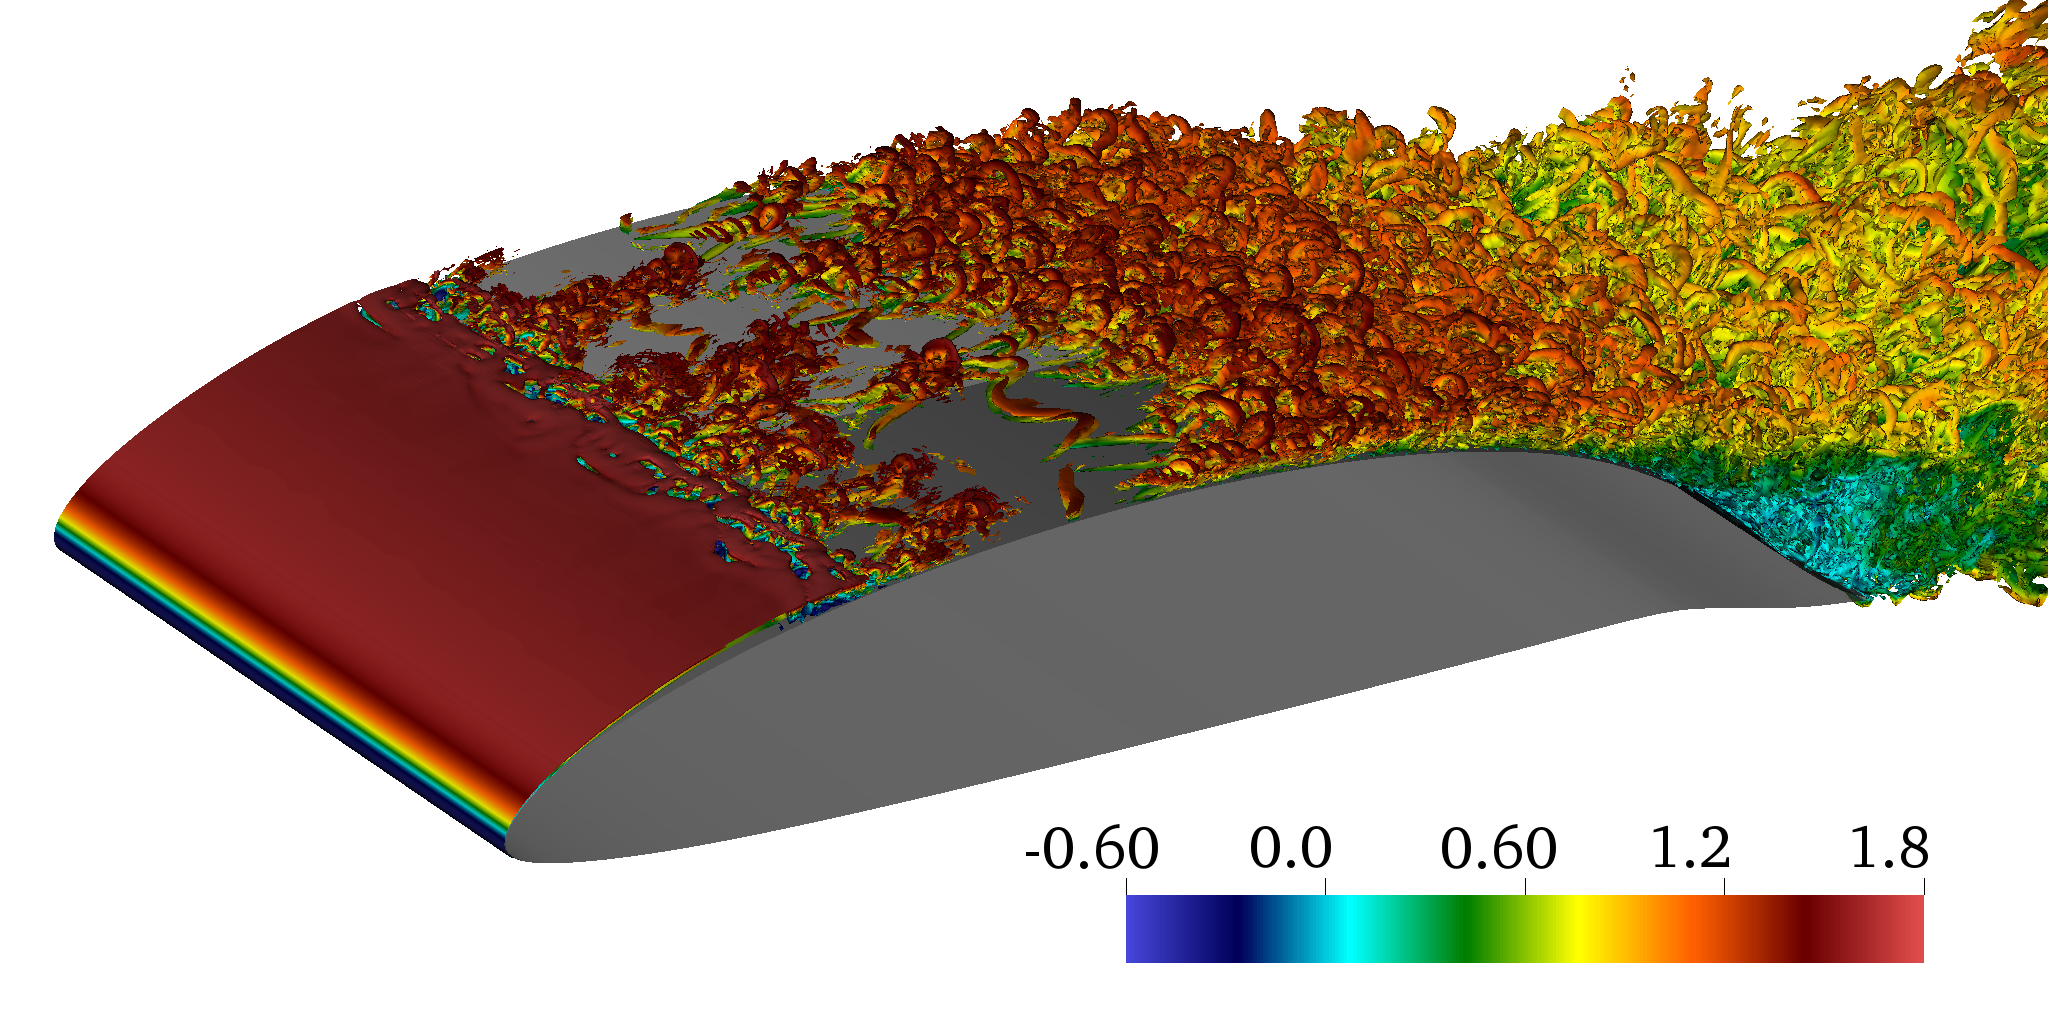
\includegraphics[width=1\textwidth]{pitch_re100k0282}
		\label{fig:upstream_2}
	\end{subfigure}
	\caption{Comparison of boundary layer transition at two different time instants of $t/T_{osc}=3.33$ (left) and $t/T_{osc}=3.35$ (right).}
	\label{fig:transition_complex}
\end{figure}

\subsection{Laminar separation bubble characteristics}

The growth of the leading-edge LSB can be quantified in terms of the maximum reverse flow observed within the recirculation region. Figure~\ref{fig:backflow_ratio} shows the absolute value of the maximum reverse flow within the circulation region normalized by the free-stream velocity at the boundary layer edge. \cite{alam00} with their local stability analysis of a two-parameter family of reverse flow profiles indicated that reverse flow intensities above $15\%$ may cause the flow to be locally absolutely unstable. With a similar analysis on a three parameter family of profiles \cite{hammond98} obtained onset of absolute instabilities at $20\%$ reverse flow velocities. The authors also performed global stability analysis on a synthetically created boundary layer with a symmetric separation bubble \citep{hammond98} and found the flow to be globally unstable for $30\%$ reverse flow velocities. In the present study the reverse flow velocities are found to be higher than $30\%$ in both the pitch cycles analyzed. Figure~\ref{fig:backflow_ratio} shows the variation of reverse flow intensity found within the leading-edge LSB. The high reverse flow state is quickly followed by flow transition over the separated shear layer of the LSB. In such a case it is possible that the leading-edge LSB changes character to become globally unstable during the pitch cycle. 
\begin{figure}
	\centering
	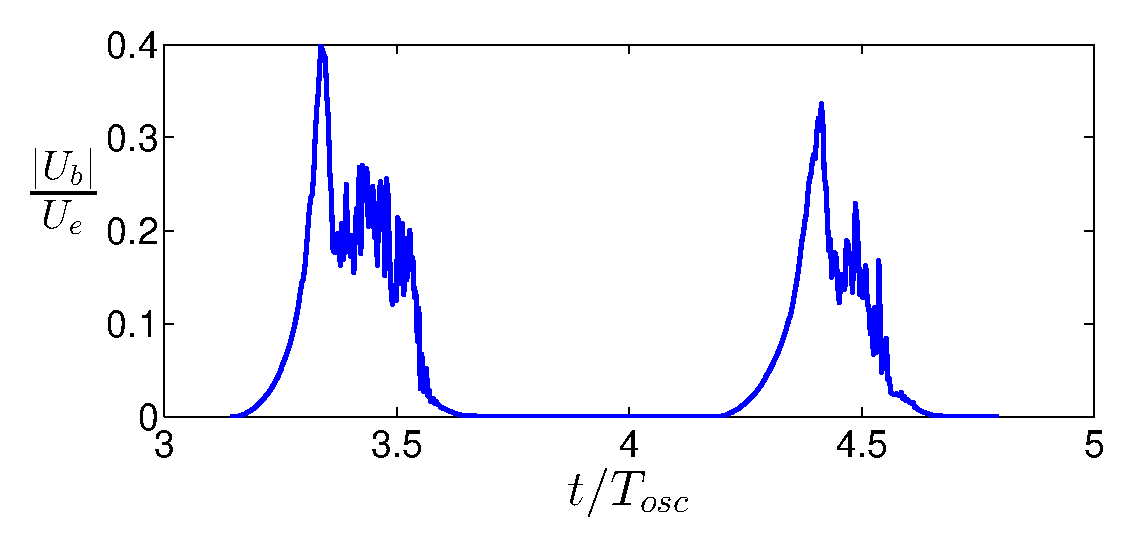
\includegraphics[width=0.8\textwidth]{backflow_ratio}
	\caption{Ratio of maximum reverse flow ($U_{b}$) in the leading-edge LSB to the boundary layer edge velocity ($U_{e}$).} 
	\label{fig:backflow_ratio}
\end{figure}

To explore such a possibility, local stability analysis of the Orr-Sommerfeld equations \citep{schmid01} is performed using the instantaneous wall-normal velocity profiles calculated as per equation~\ref{eqn:inst_q}. Several velocity profiles can be studied for their local stability characteristics. In accordance with the previous studies, we focus on the wall-normal velocity profiles which exhibit the maximum reverse flow intensity relative to the boundary layer edge velocity. The edge velocity of the local profiles was determined using the criterion of vanishing spanwise vorticity \textit{i.e.} $\overline{\omega}_{z}\approx0$. Since there is a very small but finite amount of vorticity in the far-field due to the free-stream turbulence, the criterion for boundary layer height is set as the wall-normal point where the vorticity decays to $1\%$ of its maximum value in the boundary layer. Figure~\ref{fig:bubble_profiles} shows the wall-normal velocity and vorticity profiles along with the calculated height of the boundary layer.
\begin{figure}
	\centering
	\begin{subfigure}[t]{0.48\textwidth}
		\centering
		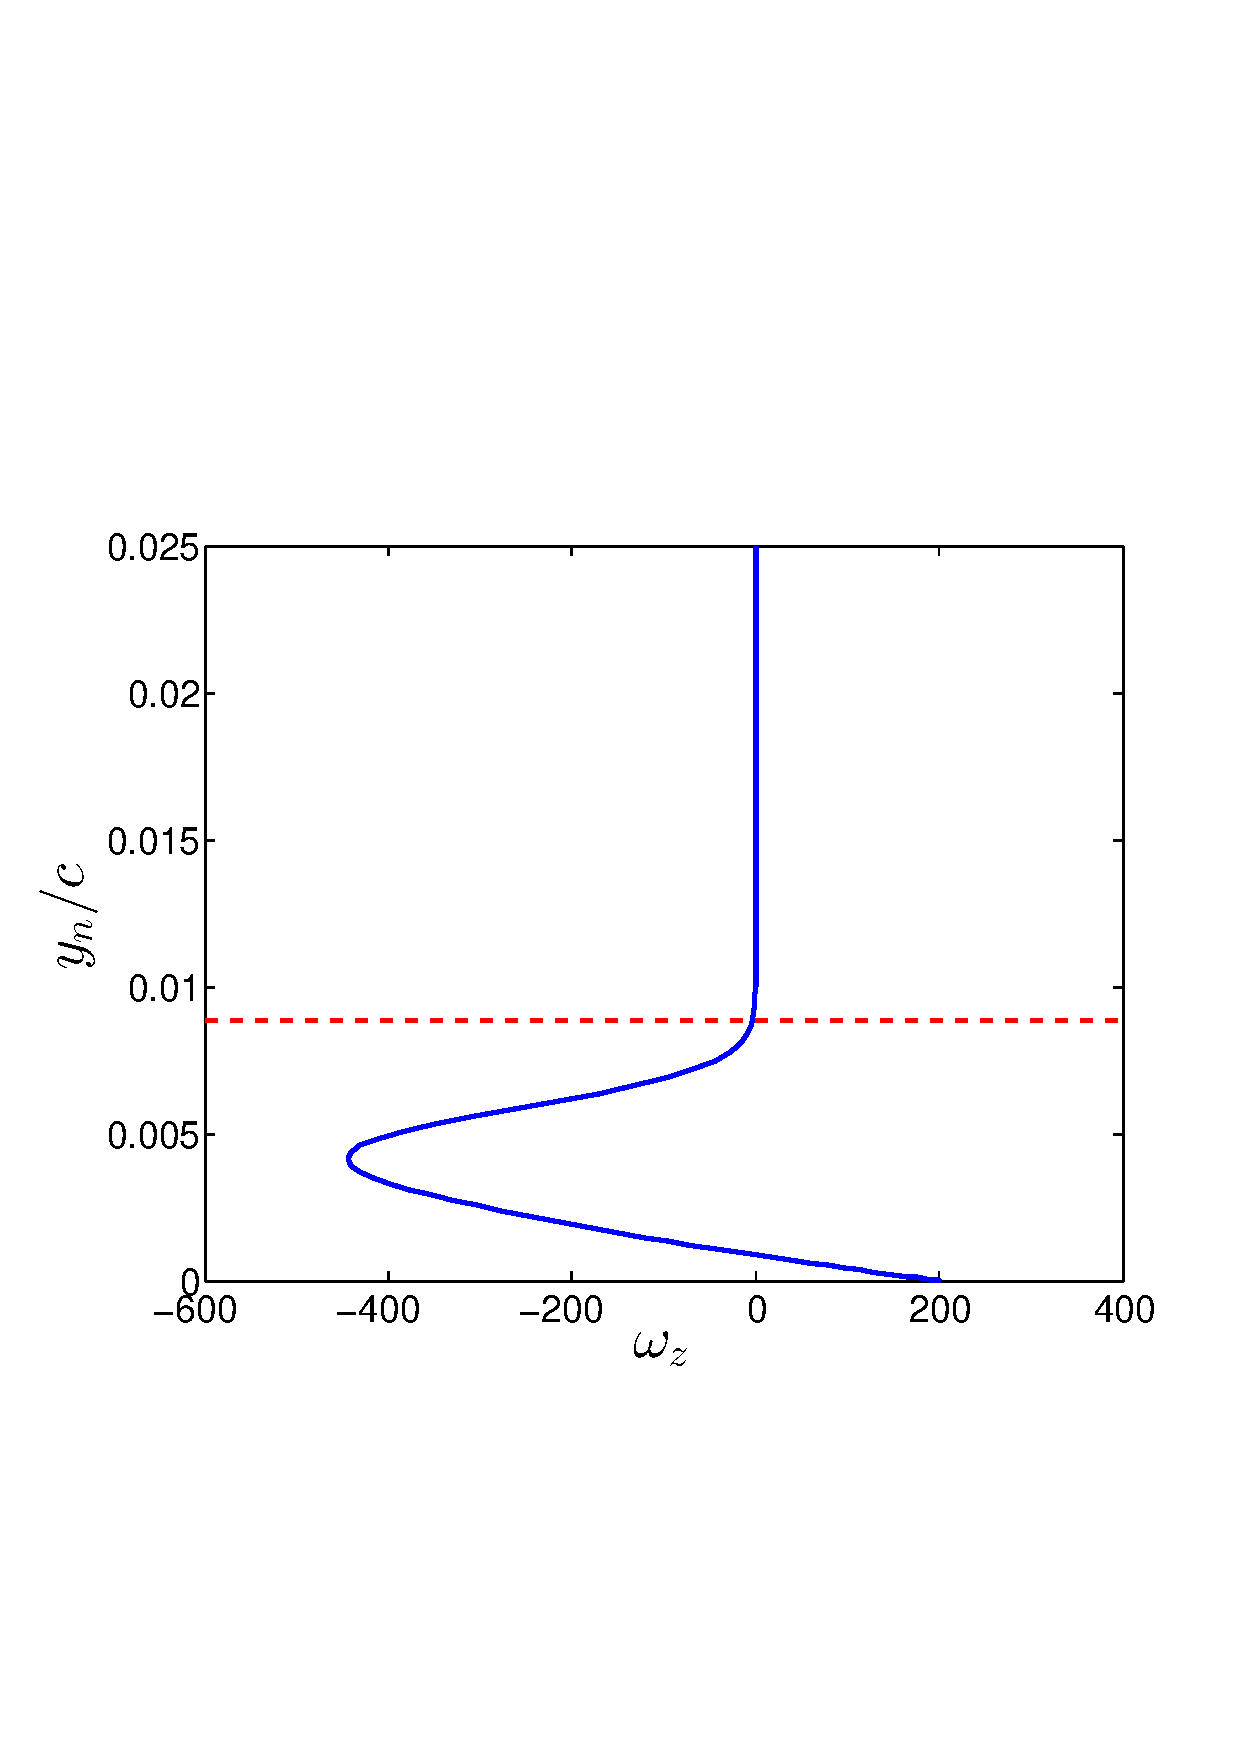
\includegraphics[width=1\textwidth]{bubble_vorticity}
	\end{subfigure}
	\begin{subfigure}[t]{0.48\textwidth}
		\centering
		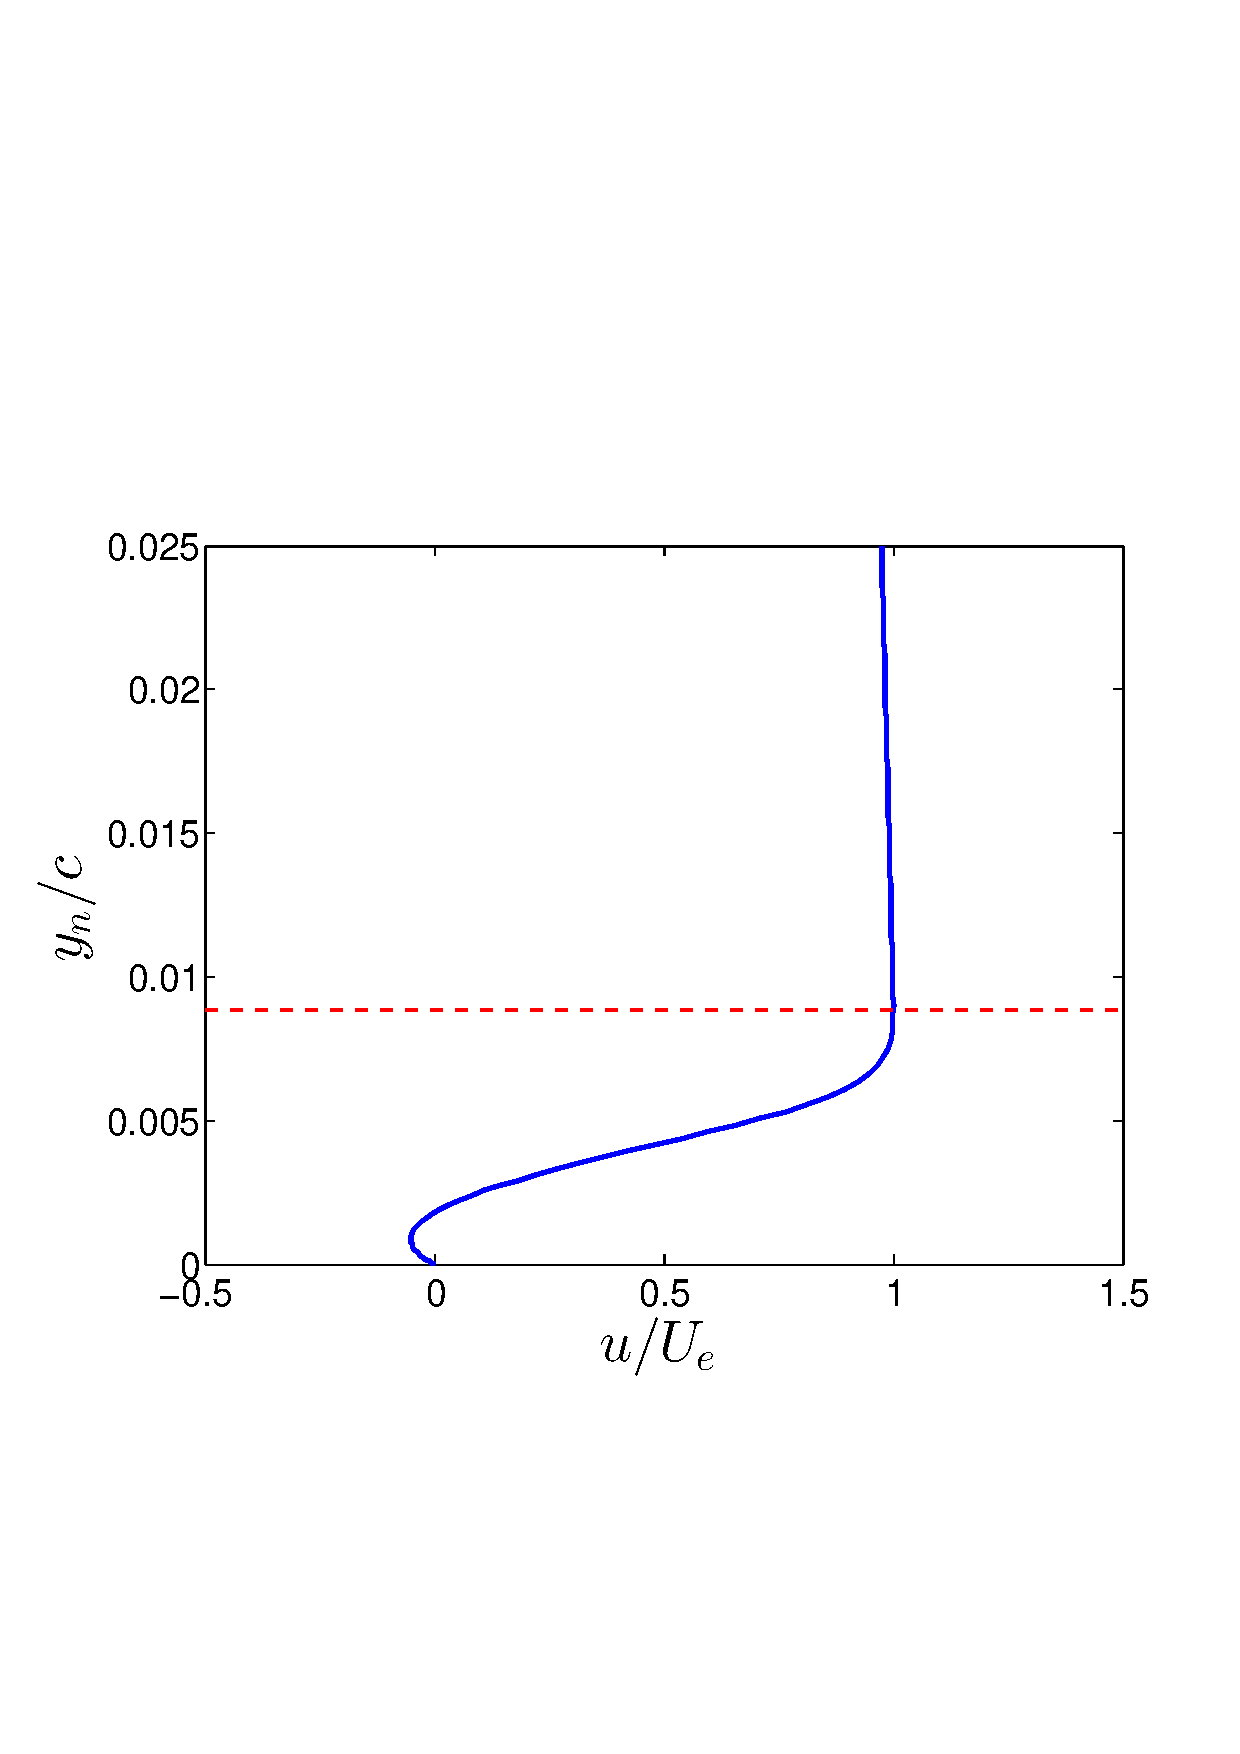
\includegraphics[width=1\textwidth]{bubble_u}
	\end{subfigure}
	\caption{Wall-normal profiles of vorticity (left) and tangential velocity (right) observed in the leading-edge LSB at $t/T_{osc}=3.25$. Dashed lines mark the boundary layer edge.}
	\label{fig:bubble_profiles}
\end{figure}

Figure~\ref{fig:bubble_lambda} shows the unstable eigenvalues obtained from a temporal stability analysis of the local velocity profiles (with varying streamwise wavenumber). The mode with the maximum amplification rate is convective in nature and this maximum amplifcation rate increases with the intensity of reverse flow found inside the leading-edge LSB. Thus the convective amplification of disturbances becomes larger as the LSB grows in size which explains the upstream motion of the transition location. In order to determine the absolute instability properties of the local velocity profiles, the cusp-map method as described by \cite{schmid01} and \cite{kupfer87} was used. Figure~\ref{fig:bubble_cusps} shows the cusps obtained in the complex frequency plane for the fourth and the fifth pitch cycles. The figure on the left shows the unstable cusp obtained in the fourth pitch cycle at $t/T_{osc}=3.32$ with a positive amplification rate of $\lambda_{i}=2.46$. On the other hand the cusp found in the fifth cycle is just marginally stable with an absolute amplification rate of $\lambda_{i}=-0.5$ at $t/T_{osc}=4.4$. Since the velocity profiles considered here are averaged values instead of stationary base-flow profiles, it is possible that small temporal variation and/or non-linear modification of the flow hides the absolute instability properties when an averaged flow-field is considered. Nonetheless the results provide a strong indication of the presence of absolute instability in the flow. 

Caution needs to be taken in the interpretation of the stability analysis. The local stability analysis using the Orr-Sommerfeld equations assumes stationary homogeneous base state. Neither of which are strictly fulfilled when using the instantaneous velocity profiles. One can compare the properties of the LSB and the instability time-scales to judge the validity of the such an analysis. The ratio of the time-period of the absolute instability ($4^{th}$ cycle) to the time period of oscillation is $0.05$, suggesting that the boundary layer would appear nearly stationary to the amplifying disturbances. For the spatial inhomogeneity, the ratio of the maximum boundary layer height to the length of the separation bubble can be used as an indicator. This ratio is equal to $\delta^{max}/L_{x}=0.03$ which suggests a weak spatial inhomogeneity. Here $\delta^{max}$ is the maximum value of the boundary layer height over the LSB and $L_{x}$ is the spatial extent of the LSB. Both the above quantities indicate the quasi-steady, homogeneous flow assumptions may be used to obtain qualitative features of the flow case. The analysis then suggests that the convective instability properties of the boundary layer become stronger as the LSB grows in size. At a certain point in the pitch cycle the LSB changes character and exhibits a region of absolute instability. This can potentially explain the emergence of two distinct transition locations. The upstream transition would be caused by the temporally growing instabilities which amplify within the region of absolute instability without being convected downstream. On the other hand spatially growing waves associated with convective instabilities would trigger transition further downstream of the LSB. The emergence of the second transition point would cause abrupt changes in the boundary layer characteristics. 

\begin{figure}
	\centering
	\begin{subfigure}[t]{0.48\textwidth}
		\centering
		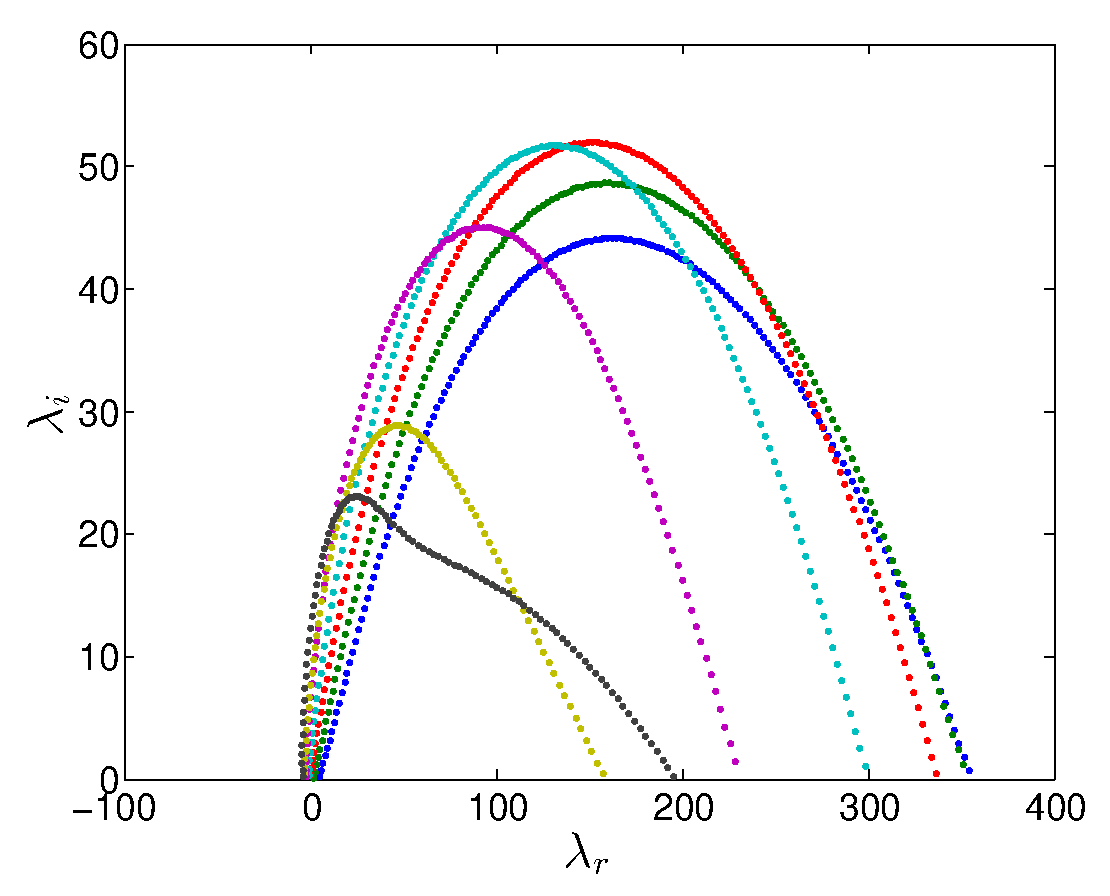
\includegraphics[width=1\textwidth]{bubble_lambda}
	\end{subfigure}
	\begin{subfigure}[t]{0.48\textwidth}
		\centering
		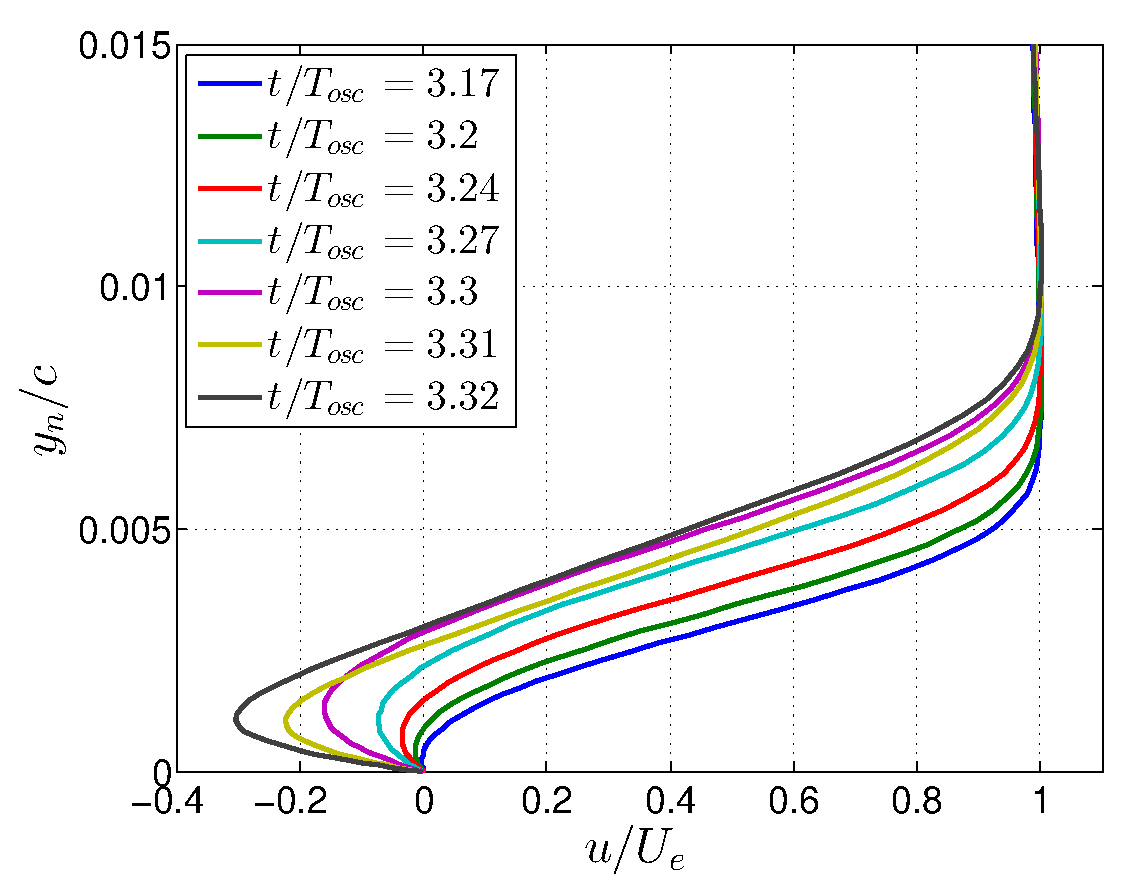
\includegraphics[width=1\textwidth]{bubble_profiles}
	\end{subfigure}
	\caption{Unstable eigenvalues (left) obtained for a temporal stability analysis for three different instantaneous velocity profiles (right). }
	\label{fig:bubble_lambda}
\end{figure}


\begin{figure}
	\centering
	\begin{subfigure}[t]{0.48\textwidth}
		\centering
		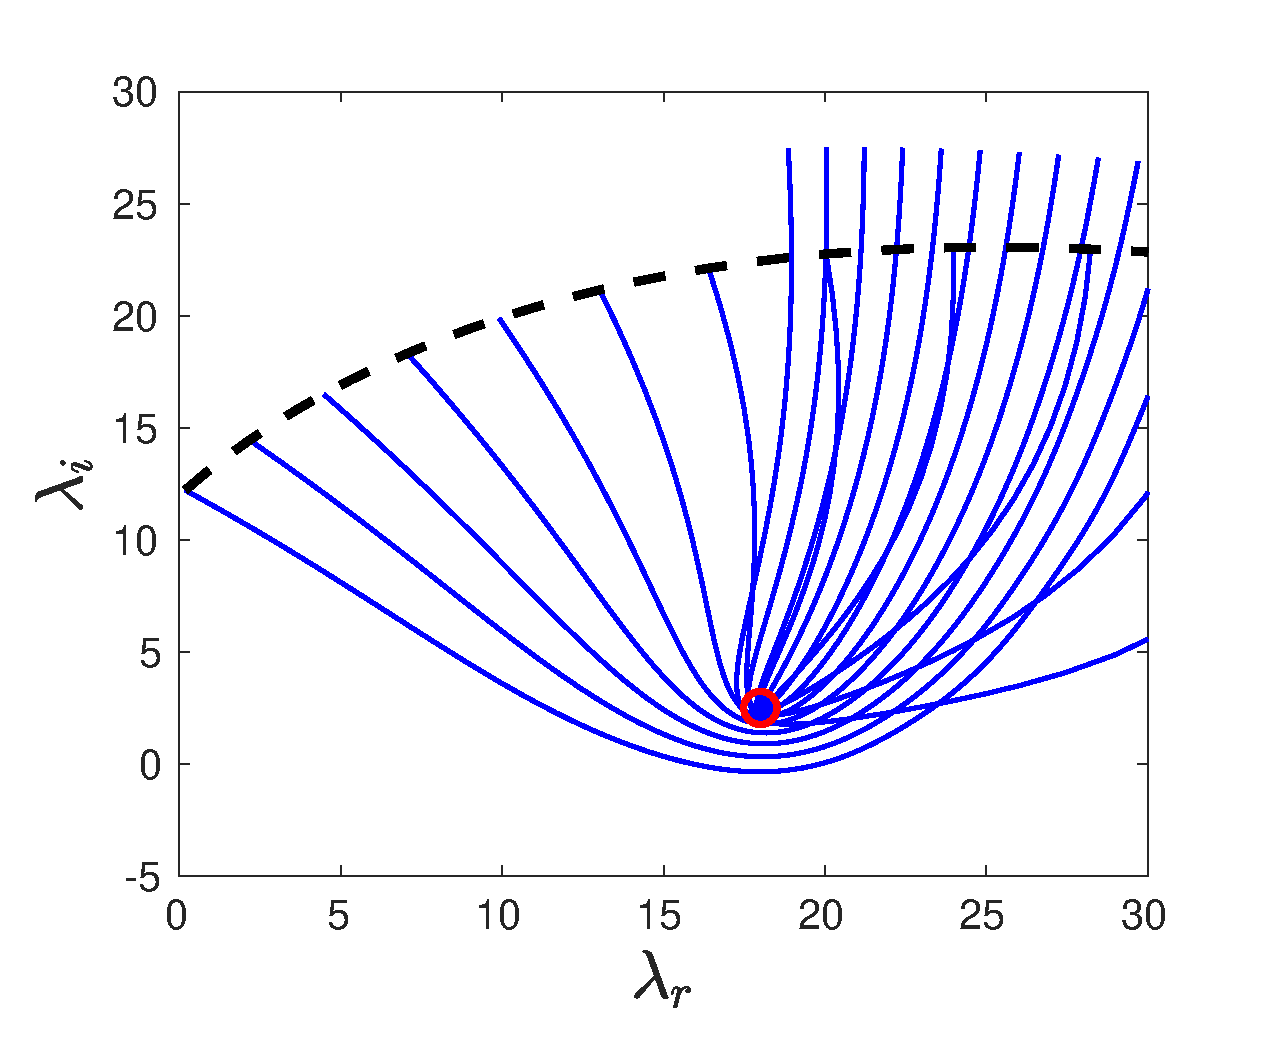
\includegraphics[width=1\textwidth]{cusp_map_88}
	\end{subfigure}
	\begin{subfigure}[t]{0.48\textwidth}
		\centering
		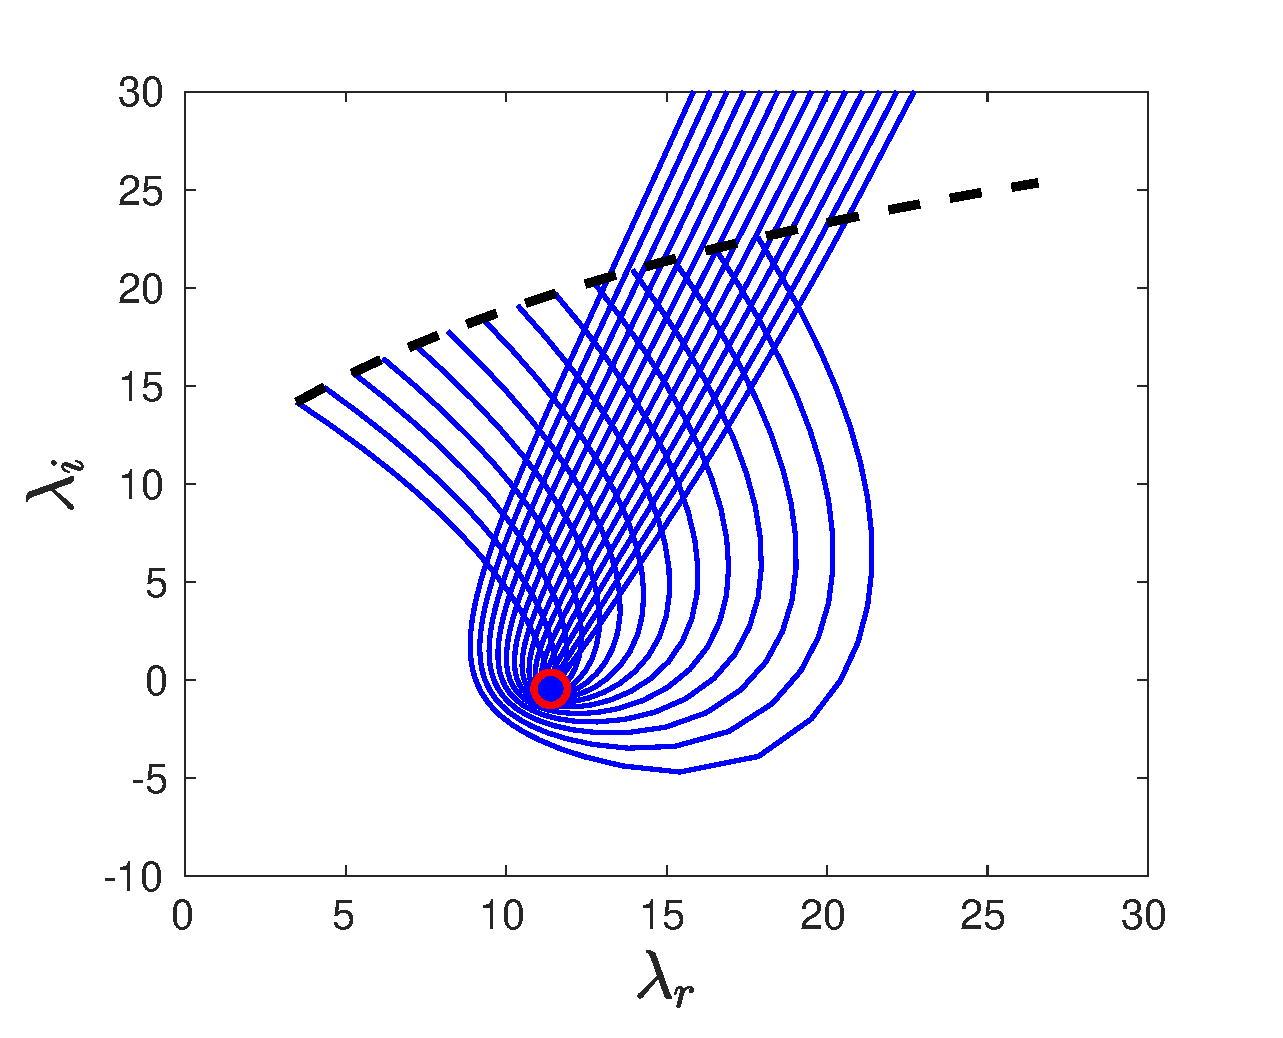
\includegraphics[width=1\textwidth]{cusp_map_427}
	\end{subfigure}
	\caption{Cusps obtained in the complex-frequency plane. An unstable cusp (left) was found in the $4^{th}$ pitch cycle and in the $5^{th}$ cycle it is marginally stable. The dashed line indicates the unstable eigenvalues obtained using real streamwise wavenumbers.}
	\label{fig:bubble_cusps}
\end{figure}

\section{Conclusion}

A relaxation-term filtering procedure is used for wall-resolved LES of flow over a pitching airfoil. Validation of the LES procedure is done in a channel flow at $Re_{\tau}=395$ and for a wing section at $Re_{c}=400,000$ and the results show a good agreement with available DNS data sets.

Flow over an airfoil is simulated using the LES procedure at a chord based Reynolds number of $Re_{c}=100,000$ within an angle of attack range where the aerodynamic forces on the airfoil exhibit sensitive dependence on the angle of attack. This sensitive dependence is captured in the steady simulations at different angles of attack with large changes in transition location within a small variation of $\alpha$.

Pitch oscillations of the airfoil within this $\alpha$ range of sensitive dependence displays a rich variety of unsteady flow phenomena. The flow goes through alternating periods of fully turbulent and laminar flow over the suction side of the airfoil with different governing mechanisms for transition through the oscillating phases. When the flow is mostly laminar over the airfoil surface it separates easily under the effect of adverse pressure gradient, forming an LSB near the trailing-edge. Flow transition occurs over this separated shear layer. As the angle of attack increases, a leading-edge LSB is formed which first excites spatially growing waves (convective instability) causing transition downstream of the LSB. The amplification rate of these spatially growing waves increases as the size of the LSB grows causing transition to move upstream. Eventually the LSB reaches a critical size and flow transition occurs abruptly on the separated shear layer of the leading-edge LSB. This is likely triggered an absolute/global instability mechanism. When transition is first triggered by this absolute instability mechanism the flow exhibits two distinct transition locations and abrupt changes in the boundary layer follow.

In the pitch-down cycle, the reverse phenomenon occurs where the leading-edge LSB shrinks in size and the region of absolute instability ceases to exit. The transition is then again governed by spatially amplifying waves. The spatial amplification rate now reduces as the LSB shrinks and transition moves downstream. The flow thus goes through states of convective and absolute instability, causing a continuous change in the transition location. The upstream and downstream velocities of the transition point movement however are vastly different, with an average upstream velocity being around $V^{tr}_{u}\approx-0.60$ and a much slower downstream velocity of $V^{tr}_{d}\approx0.17$. This asymmetry is yet to be investigated, but may be an important parameter in unsteady turbulence modeling.

\section*{Acknowledgement} 

The computations were performed on resources provided by the Swedish National Infrastructure for Computing (SNIC) at the PDC Center for High Performance Computing at the Royal Institute of Technology (KTH). The work was partially funded by European Research Council under grant agreement 694452-TRANSEP-ERC-2015-AdG. The work was also partially funded by Vinnova through the NFFP project UMTAPS, with grant number 2014-00933. We would like to thank Dr. David Eller and Mikaela Lokatt for providing us with the NLF design and the numerous discussions on different aerodynamic aspects of the project.


%%%%%%%%%%%%%%%%%%%%%%%%%%%%%%%%%%%%%%%%%%%%%%%%%%%%%%%%%%%%%%%%%%%%%%
%\FloatBarrier

%%%%%%%%%%%%%%%%%%%%%%%%%%%%%%%%%%%%%%%%%%%%%%%%%%%%%%%%%%%%%%%%%%%%%%
%\bibliographystyle{tsfp}
%\bibliography{tsfp}
% In this example, BibTeX is used
% For users not familiar with LaTeX, the bibliography can be typed in directly. In this case, comment the two lines above.



%\end{document}
